%!TEX encoding = UTF-8 

%\documentclass{book}
\documentclass[a4paper,titlepage]{book} 

\usepackage[italian,portuguese,english]{babel}
% or just declare english, then use \begin{otherlanguage*}{italian}text\end{otherlanguage*}
%\usepackage[english]{babel}		%	different languages (last one is the main one)
							
\usepackage[utf8]{inputenc}		%	type accented characters in source
%\usepackage[smaller]{acronym}			%	acronyms
\usepackage{acronym}			%	acronyms
\usepackage{algorithm}			%	float wrapper for algorithms - load before hyperref
\usepackage{algorithmic}			%	describe algorithms - load after hyperref?
\usepackage{graphicx}			%	images
\usepackage{amsmath}			%	mathematics
\usepackage{booktabs}			%	tables
\usepackage{fancyhdr}			%	to use \abstract with book documentclass
\newcommand{\fncyblank}{\fancyhf{}}
\newenvironment{abstract}%
{\clearpage\fncyblank\null\vfill\begin{center}% % not \cleardoublepage
\bfseries\abstractname\end{center}}%
{\vfill\null}
\usepackage{frontespizio}		%	Italian thesis frontispiece
\usepackage{leftidx}				%	left indexes
%\usepackage{listings}			%	code listings
\usepackage{makeidx}			%	enable index
%\usepackage{microtype}		%	improves filling of rows
\usepackage{pdfpages}			%	insert PDFs
\usepackage[resetlabels]{multibib}	%	multiple bibliographies
\newcites{web}{Online references}	%	create "webography"
\usepackage{subfig}				%	align figures and tables
%\usepackage{wrapfig}			%	wrap text around an image
\usepackage{hyperref}			%	\href{url}{text} hyperlinks in cross-refs
\hypersetup{%
	pdfauthor=Giovanni Saponaro,
	pdftitle=Object Manipulation from Simplified Visual Cues,
	pdfsubject=MSc Thesis,
	%colorlinks,%
	%citecolor=black,%
	%filecolor=black,%
	%linkcolor=black,%
	%urlcolor=black,%
	%plainpages,
	%plainpages=false,
	%pdfpagelabels
}

% make \marginpar size smaller than the default
\setlength{\marginparwidth}{1.2in}
\let\oldmarginpar\marginpar
\renewcommand\marginpar[1]{\-\oldmarginpar[\raggedleft\footnotesize #1]%
{\raggedright\footnotesize #1}}

\newcommand{\degree}{\ensuremath{^\circ}}
% centred horizontal line to be used before the first \midrule in tables
\newcommand{\otoprule}{\midrule[\heavyrulewidth]}
\newcommand{\theHalgorithm}{\arabic{algorithm}} % fixes algorithms-hyperref conflict

\newenvironment{eqsystem}% 
{\left\lbrace\begin{array}{@{}l@{}}}% 
{\end{array}\right.}

\makeindex

%%%%%%%%%
\begin{document}
%%%%%%%%%

\begin{frontespizio}
%\Universita[Sapienza]{Roma} % no: aggiunge la scritta "Universit� degli studi di"
\Istituzione{Sapienza -- Universit\`a di Roma} % OK: non aggiunge scritte prima
\Logo{figures/ML_tratto_rosso}
\Facolta{Ingegneria} 
\Corso[Laurea Specialistica]{Ingegneria Informatica} 
\Annoaccademico{2007--2008} 
\Titoletto{Tesi di Laurea Specialistica} 
\Titolo{Object Manipulation from Simplified Visual Cues} 
%\Sottotitolo{} 
\Candidato{Giovanni Saponaro} 
\Relatore{Prof. Daniele Nardi} 
\Correlatore{Prof. Alexandre Bernardino} 
\end{frontespizio}

%%%%%%
\frontmatter
%%%%%%

% 1. frontispiece (OK, already taken care of by frontespizio class)

% 2. dedication (dedica)

% 3. abstract (sommario)
%!TEX encoding = UTF-8 

\selectlanguage{italian}%
\begin{abstract}
La robotica umanoide in generale, e l'interazione uomo--robot in particolare, stanno oggigiorno guadagnando nuovi e vasti campi applicativi: la robotica si diffonde sempre di pi\`u nella nostra vita. Una delle azioni che i robot umanoidi devono poter eseguire \`e la manipolazione di cose (avvicinare le braccia agli oggetti, afferrarli e spostarli). Tuttavia, per poter fare ci\`o un robot deve prima di tutto possedere della \emph{conoscenza} sull'oggetto da manipolare e sulla sua posizione nello spazio. Questo aspetto si pu\`o realizzare con un approccio percettivo.

Il sistema sviluppato in questo lavoro di tesi \`e basato sul \emph{tracker} visuale CAMSHIFT e su una tecnica di ricostruzione 3D che fornisce informazioni su posizione e orientamento di un oggetto generico (senza modelli geometrici) che si muove nel campo visivo di una piattaforma robotica umanoide. Un oggetto \`e percepito in maniera \emph{semplificata}: viene approssimato come l'ellisse che racchiude meglio l'oggetto stesso.

Una volta calcolata la posizione corrente di un oggetto situato di fronte al robot, \`e possibile realizzare il \emph{reaching} (avvicinamento del braccio all'oggetto). In questa tesi vengono discussi esperimenti ottenuti col braccio robotico della piattaforma di sviluppo adottata.
\end{abstract}

\selectlanguage{english}%
\begin{abstract}
Humanoid robotics in general, and human--robot interaction in particular, is gaining new, extensive fields of application, as it gradually becomes pervasive in our daily life. One of the actions that humanoid robots must perform is the manipulation of things (reaching their arms for objects, grasping and moving them). However, in order to do this, a robot must first have acquired some \emph{knowledge} about the target object and its position in space. This can be accomplished with a perceptual approach.

The developed system described in this thesis is based on the CAMSHIFT visual tracker and on a 3D reconstruction technique, providing information about position and orientation of a generic, model-free object that moves in the field of view of a humanoid robot platform. An object is perceived in a \emph{simplified} way, by approximating it with its best-fit enclosing ellipse.

After having computed where an object is currently placed in front of it, the robotic platform can perform reaching tasks. Experiments obtained with the robot arm of the adopted platform are discussed.
\end{abstract}


% 4. acknowledgements
%!TEX encoding = UTF-8

\chapter*{Acknowledgements}

% get inspiration from
% http://www.robots.ox.ac.uk/~teo/thesis/Thesis/deCampos3DHandTracking1.pdf

First of all, I would like to thank my daily supervisor in this project for his uninterrupted support and patience during my eight months of stay in VisLab and Institute for Systems and Robotics, Instituto Superior T\'{e}cnico, Lisbon. Thank you very much, Prof.~Alexandre~Bernardino. That, plus\dots{} passionately discussing algorithms while eating a Portuguese \emph{doce} and sipping a coffee together (several times) is priceless.

I also wish to express my gratitude to my home advisor: Prof.~Daniele~Nardi of Sapienza University of Rome. Not only has he provided me with the chance to do my thesis research abroad, but he has been helpful, encouraging and available for suggestions at all times.

I would like to thank Prof.~Jos\'{e}~Santos-Victor of Instituto Superior T\'{e}cnico for his confidence in hosting me, and for making VisLab such an enjoyable environment to work at, ultimately making it a breeze to do research there. %

This work was partially supported by EC Project IST-004370 RobotCub and by the Portuguese Government~--~\begin{otherlanguage*}{portuguese}Funda\c{c}\~{a}o para a Ci\^{e}ncia e Tecnologia\end{otherlanguage*} (ISR/IST pluriannual funding) through the POS\_Conhecimento Program that includes FEDER funds. This is gratefully acknowledged.

\bigskip

In Lisbon I found plenty of nice people since day one. I am glad to have met the \emph{Italian gang} of IST, dearest friends and valued teachers to me: Alessio, Giampiero and Matteo. And then I certainly wish to thank many more colleagues for the fruitful discussions that ensued and for the fun (apologies if I forgot anybody): Christian, Daniel, Daniela, Dario, Prof.~Gaspar, Ivana, Jonas the Superschwiizer, Jonas the Swede, Luis\~{a}o, L.~Vargas, Manuel, Marco, M\'ario, Matthijs, Plinio, Ricardo, Rub\'{e}n, Samuel, Verica.

Thank you Aleka, Andrea, Patty, Sabrina, Valentin and everybody else back from my Erasmus year. Cheers to Cimpe and Claudione, crazy Portugal-lovers. Oh, thanks to PierFrok for the tip.
% o PierPal?

% Vicky, Lisa, Tomas? Toni, S�rgio

\begin{otherlanguage*}{portuguese}
Nico (e Tigas), obrigado por tudo, desde 2005\copyright.
Obrigado \`{a} \emph{trindade}: Carmen, Joana, Lara, Leonor. Agrade\c{c}o tamb\'{e}m ao Gustavo, ao Pi\c{c}arra, ao Paulo e a todos os portugueses que andam por Roma.
\end{otherlanguage*}

\bigskip

\begin{otherlanguage*}{italian}
Naturalmente grazie a tutti coloro con cui ho condiviso esperienze in Italia. A Balerio per l'amicizia antica. A Sofia, \emph{sister of a lifetime}. Ai compagni di scuola: Ilardo, Il Giulio, Jessica, Lorenzo, Nausicaa, Valerione Picchiassi. Ai compagni di universit\`{a}: la \emph{crew} ``Gli anni '12'' e lo staff di foruming.

% Flo e famiglia?

Grazie ad Aurora, a Ludovico e ai gatti tutti: anche se preferisco i cani, faccio un'eccezione.

Grazie a tutti gli altri amici relativamente recenti ma gi\`{a} ottimi e abbondanti: Aldo Rock, Mauro, Simone, Riccardo.

\bigskip

E poi, grazie davvero a \emph{tutta} la mia famiglia. A mia madre Paola e a mio padre Francesco per il loro amore infinito. A mio fratello Davide che \`{e} sempre stato fonte di ispirazione; ad Arianna e a Carlo.
\end{otherlanguage*}

% 5. table of contents (indice) and other lists
\tableofcontents
\listoffigures
\listoftables
\listofalgorithms % ?

% 6. list of acronyms, abbreviations and notation
%!TEX encoding = UTF-8 

\chapter*{List of Acronyms and Abbreviations}

\begin{acronym}[CAMSHIFT]
\acro{ADC}{Analogue-to-Digital Converter}

\acro{AI}{Artificial Intelligence}

\acro{API}{Application Programming Interface}

\acro{BLAS}{Basic Linear Algebra Subprograms}

\acro{CAMSHIFT}{Continuously Adaptive Mean Shift}

\acro{CCD}{Charge-Coupled Device}

\acro{CLAWAR}{Climbing and Walking Robots and the Support Technologies for Mobile Machines}

\acro{CV}{Computer Vision}

\acro{CMY}{Cyan Magenta Yellow}

\acro{DH}{Denavit-Hartenberg}

\acro{DOF}{Degree of Freedom}

\acro{DSP}{Digital Signal Processor}

\acro{EM}{Expectation Maximization}

\acro{FPGA}{Field-Programmable Gate Array}

\acro{FPS}{Frames per Second}

\acro{GSL}{GNU Scientific Library}

%\acro{HSL}{hue, saturation, lightness}

\acro{HSV}{Hue Saturation Value}

\acro{IBVS}{Image-Based Visual Servoing}

\acro{IPC}{Inter-Process Communication}

\acro{MDH}{Modified Denavit-Hartenberg}

\acro{NMC}{Networked Modular Control}

\acro{ROI}{Region of Interest}

\acro{PBVS}{Position-Based Visual Servoing}

\acro{PSC}{Propagation of Surfaces under Curvature}

\acro{PUI}{Perceptual User Interface}

\acro{RGB}{Red Green Blue}

\acro{RobotCub}{Robotic Open-Architecture Technology for Cognition, Understanding and Behaviour}

\acro{SDH}{Standard Denavit-Hartenberg}

\acro{SOM}{Self-Organizing Map}

\acro{YARP}{Yet Another Robot Platform}
\end{acronym}


%%%%%%
\mainmatter
%%%%%%

% 7. introduction (prefazione) with many sections => mainmatter
%!TEX encoding = UTF-8 

% ugly and possibly dangerous command
%\setcounter{page}{15}

\chapter{Introduction}

%%%%%%%%%%%
\section{Motivation}

A current field of research in humanoid robotics\index{humanoid robotics} is the study of \emph{interactions} between a robot and its human users, focusing on topics such as perception\index{perception}, learning and imitation. Neurosciences\index{neurosciences} and developmental psychology\index{developmental psychology|see{psychology}}\index{psychology}, which study the inner mechanisms of the human brain, also contribute to these matters as they try to understand key cognitive\index{cognition} issues: how to learn sensory-motor coordination\index{sensory-motor coordination}, which properties of observed objects or of the world we learn, how human beings imitate\index{imitation} each other, and how they recognize actions.

The reason why interactions are relevant and worth studying in robotics is twofold. First, they allow us to progress within the underlying scientific disciplines: robotics, image processing, \ac{CV}, \ac{AI}, signal processing and control theory.

Secondly, by improving human-robot interactions\index{interactions} and better understanding our brain\index{cognition}, we also contribute to specific applications that have an increasing \emph{social impact}, namely rescue operations, emergencies, visual monitoring of urban areas, as well as robotic assistants that improve quality of life for the elderly or disabled people~\cite{hu:2007}.

\begin{figure}
\centering
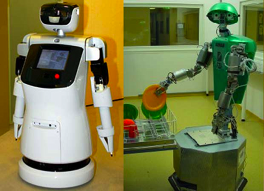
\includegraphics{figures/service_robots}
\caption[Example of service robots]{Two examples of service robots, built by the University of Karlsruhe (Germany) and Fujitsu, respectively.}
\label{img:service_robots}
\end{figure}

Grasping\index{grasping} and manipulation\index{manipulation} are among the most fundamental tasks to be considered in humanoid robotics\index{humanoid robotics}. Fig.~\ref{img:service_robots} shows two examples of service robotics platforms that possess enough tools, appliances and flexibility to potentially adapt to human tasks\index{imitation}.

Just like humans distinguish themselves from other animals by having highly skilled hands, so can humanoid robots: dexterous ability must be considered as a key component in practical applications such as service robotics or personal robot assistants.

The high dexterity that characterizes human manipulation does not come for granted at birth. Instead, it arises gradually during a complex developmental process which spans different stages. After recognizing things surrounding them by the means of \emph{vision}, babies first attempt to reach for these things, with a very limited precision. Then, at some point they start to adapt their hands to the shape of objects, initially letting these objects fall on the ground because of incorrect grasping procedures. Only after some years are they finally able to master their arm and hand skills.

Furthermore, perception\index{perception} develops in parallel with these manipulation\index{manipulation} skills, in order to incrementally increase the performance in detecting and measuring those object features that are important for touching, grasping\index{grasping} and holding something. Along time, interactions with objects of diverse shapes are successfully performed by applying various possible reaching\index{reaching} and manipulation techniques. Salient\index{saliency} effects are produced (e.g., an object moves, it is deformed, or it makes a sound when squeezed), perceived and associated to actions. An agent thus learns object affordances~\cite{montesano:2008}\index{object affordances}\index{affordances|see{object affordances}}, i.e., the relationships among a certain manipulation\index{manipulation} action, the physical characteristics of the object involved, and the observed effects. The way of reaching for an object evolves from a purely position-based mechanism to a complex behaviour which depends on target size, shape, orientation\index{orientation}, intended usage and desired effect.

Framed within the \ac{RobotCub} Project~\cite{metta:2005}\index{RobotCub}, this thesis aims at providing \emph{simple} 3D object perception\index{perception} for enabling the development of manipulation\index{manipulation} skills in a humanoid robot\index{humanoid robotics}, by approximating a perceived object with its best-fit enclosing ellipse\index{ellipse}. 

This work addresses the problem of reaching\index{reaching} for an object and preparing the grasping\index{grasping} action, according to the \emph{orientation}\index{orientation} of the objects to interact with. The proposed technique is not intended to have very accurate measurements of object and hand postures, but merely the necessary quality to allow for successful object--hand interactions. Precise manipulation\index{manipulation} needs to emerge from experience by optimizing action parameters as a function of the observed effects. To have a simple enough model of object and hand shapes, they are approximated as 2D ellipses\index{ellipse} located in a 3D space. An underlying assumption is that objects have a sufficiently \emph{distinct colour}, in order to facilitate segmentation\index{image segmentation} from the image background. Perception\index{perception} of object orientation\index{orientation} in 3D is provided by the second-order moments of the segmented areas in left and right images, acquired by a humanoid robot active vision head.

This thesis will describe: the humanoid robot platform ``Baltazar'' that was used for research and tests, the adopted \ac{CV} techniques, a simple method to estimate the 3D orientation of a target object, strategies for the reaching and grasping tasks, experimental results and future work.

%%%%%%%%%%%%%%%%%%%%%%%%%%%%%%%%%%%%%%%
\section[RobotCub]{RobotCub and the Development of a Cognitive Humanoid Robot}
\index{RobotCub}

\begin{figure}
\centering
\subfloat[][RobotCub Consortium logo.]
{
\includegraphics[width=.55\columnwidth]{figures/robotcub} \label{img:robotcub} } \quad
% %necessary to prevent line break
\subfloat[][The iCub robot platform standing.]
{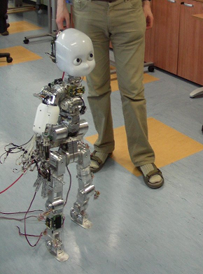
\includegraphics[width=.35\columnwidth]{figures/icub_standing} \label{img:icub_standing} }
\caption[RobotCub logo and iCub baby robot prototype]{RobotCub logo and a prototype of its baby robot prototype, the iCub.}
\label{fig:robotcub-icub}
\end{figure}

The \ac{RobotCub} Consortium~\cite{link:robotcub}\index{RobotCub} is a five-year-long project, funded by the European Commission through Unit E5 (``Cognition'') of the Information Society Technologies priority of the Sixth Framework Programme (FP6). 

\ac{RobotCub} is a project to study cognition through robotics. Its objective is to create a completely open design for a humanoid robot --- ``open hardware,
open software, open mind''. All the \ac{RobotCub} hardware designs and software are free and open source\index{open source}. The \ac{RobotCub} Consortium is composed of 16 partners: 11 from Europe, 3 from Japan and 2 from the USA. LIRA-Lab~\cite{link:liralab} at the University of Genoa, Italy, is the coordinator.

Inspired by recent results in neurosciences\index{neurosciences} and developmental~psychology\index{psychology}, the objective of \ac{RobotCub} is to build an open-source humanoid platform for original research on cognitive robotics, with a focus on developmental aspects. One of the tenets of the project is that manipulation\index{manipulation} plays a key role in the development of cognitive ability.

% balta_workspace is not used atm

%\begin{figure}
%\centering
%\subfloat[][The iCub robot platform standing.]
%{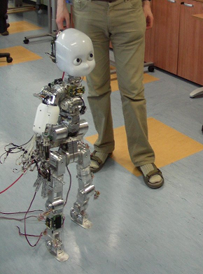
\includegraphics[width=.35\columnwidth]{figures/icub_standing} \label{img:icub_standing} } \quad
% %necessary to prevent line break
%\subfloat[][Baltazar robot platform in its workspace.]
%{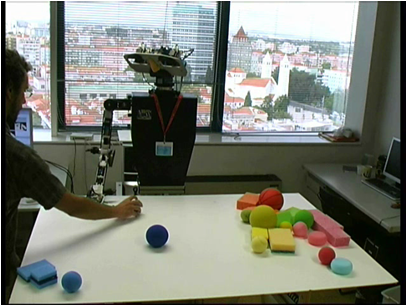
\includegraphics[width=.55\columnwidth]{figures/balta_workspace} \label{img:balta_workspace} }
%\end{figure}

The iCub\index{iCub}\label{icub} is a humanoid baby robot designed by the \ac{RobotCub} consortium. The iCub, shown in Fig.~\ref{img:icub_standing}, is a full humanoid robot the size of a two-year-old child. Its total height is around 90 cm, and it has 53 \acp{DOF}, including articulated hands to be used for manipulation\index{manipulation} and gesturing; in addition, the iCub is equipped with an inertial system in its hand, stereo audition, and the ability to perform facial expressions.

At the time of writing this thesis, a study is being conducted for determining if and how many \acp{DOF} are minimally required to produce and generate plausible facial expressions. The iCub\index{iCub} robot should eventually be able to crawl and sit (to free the hands from supporting the body) and autonomously transition from crawling to sitting and vice-versa. 

This thesis work was carried out at the Computer and Robot Vision Laboratory~\cite{link:vislab}, Institute for Systems and Robotics, IST, Lisbon (Portugal) during 2008. At the time of working on this project, the arm-hand system of a full iCub prototype was still being assembled. Therefore, for this work another humanoid robot platform was used: Baltazar~\cite{lopes:2004, lopes:2007}\index{Baltazar}. It consists of a robotic torso and a binocular head, built with the aim of understanding and performing human-like gestures, mainly for biologically inspired research.

%%%%%%%%%%%%%%%
\section{Thesis Background}

Manipulation skills\index{manipulation} at macro- and micro-scales are very important requirements for robot applications. This is valid both in industrial robotics\index{industrial robotics} and in less-traditional fields. As far as industry is concerned, robot manipulators hold a key role in many scenarios; to name a few:
\begin{itemize}
\item handling;

\item food;

\item fabrics;

\item leather.
\end{itemize}

Similarly, in less structured domains of robotics, manipulation still play a relevant part:
\begin{itemize}
\item surgery;

\item space;

\item undersea.
\end{itemize}

Manipulation and grasping systems are thus a vital part of industrial, service and personal robotics, they are employed in various applications and environments, not just in advanced manufacturing automation as one may intuitively think.

\begin{figure}
\centering
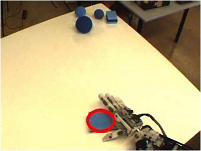
\includegraphics{figures/balta_grasping}
\caption[Baltazar humanoid robot and its workspace]{Humanoid robot Baltazar operating in its workspace, as seen from one of its cameras. The anthropomorphic hand of Baltazar is reaching for a visually-tracked object and is about to grasp it.}
\label{img:balta_grasping}
\end{figure}

Actuating a robotic limb is not merely commanding it to a given position: the issue is also where and how to move it, and for this purpose \ac{CV} (the ability for machines to understand images) is a powerful tool that can assist humanoid robotics broadly. In particular, \ac{CV} is used for robot manipulation tasks: reaching for something, touching or grasping it.

A major difficulty for humanoid robots in order to successfully perform a grasping task is the \emph{variety of objects} they have to interact with: a robot should be able to see and understand any shape and size, including never-before-seen objects. To do this, deploying simple \emph{model-free} methods (i.e., not enforcing any model) is often the sensible choice to follow, including in the approach presented in this thesis.

In particular, our objective is to approximate an object positioned in front of a humanoid robot with its smallest \emph{enclosing ellipse}\index{ellipse}. In addition, the target object may not necessarily be static, so the developed techniques must also cope with following where this target is moving. This is done by the means of \ac{CAMSHIFT} trackers.

A computer vision technique to estimate the 3D position and orientation of a moving target object placed in front of a humanoid robot, equipped with a stereo rig, will be presented. The information inferred will subsequently be used by the robot to better \emph{interact} with the object, that is, to manipulate it with its arm: an approach for real-time preparation of grasping tasks is described, based on the low-order moments of the target's shape on a stereo pair of images acquired by an active vision head.

\label{intro:reaching_phases}
To reach for an object\index{reaching}, two distinct phases are considered~\cite{lopes:2007}:
\begin{enumerate}
\item an open-loop ballistic phase to bring the manipulator to the vicinity of the target, whenever the robot hand is not visible in the robot's cameras;

\item a closed-loop visually controlled phase to accomplish the final alignment to the grasping position.
\end{enumerate}

The open-loop phase (reaching preparation) requires the knowledge of the robot's inverse kinematics and a 3D reconstruction of the target's posture. The target position is acquired by the camera system, where the hand position is measured by the robot arm joint encoders. Because these positions are measured by different sensory systems, the open-loop phase is subject to mechanical calibration errors. The second phase (grasping preparation), operates when the robot hand is in the visible workspace. 3D position and orientation of target and hand are estimated in a form suitable for \acl{PBVS} (\acs{PBVS})~\cite{chaumette:visual1, hutchinson:1996}. The goal is to make the hand align its posture with respect to the object. Since both target and hand postures are estimated in the same reference frame, this methodology is not prone to significant mechanical calibration errors.

%%%%%%%%%%%%%%%%
\section{Problem Statement}

The objective is to estimate the 3D position and orientation of an object placed in front of a humanoid robot, in order for make it possible to interact and manipulate such object. This estimation is done in two visual processing steps: tracking the object shape as it (possibly) moves within the robot stereo cameras' 2D vision, then combining the inferred information through 3D reconstruction methods.

Computation must be real-time, so that the understanding of a dynamic scene and the interactions with objects are accurate but also usable in practical experiments. This constraint calls for a simplified, model-free vision approach. An object position and orientation will be approximated with its best-fit enclosing ellipse.

Furthermore, the employed software components must be clearly decoupled, in order to make it possible to adapt them to other robotic platforms and scenarios (such as a full iCub robot; see p.~\pageref{icub}).

Finally, the geometric measurements acquired so far should to be used for the two phases of a reaching task, necessary for object manipulation: (i) an initial phase whereby the robot positions its hand close to the target with an appropriate hand orientation, and (ii) a final phase where a precise hand-to-target positioning is performed using Visual~Servoing methods.

%%%%%%%%%%%%%%
\section{Thesis Structure}

The thesis is organized as follows:

%
\begin{itemize}
\item Chapter~\ref{chap:related_work} lists the existing techniques for segmentation, stereo~vision (in particular 3D reconstruction) and manipulation tasks for humanoid robots;

\item Chapter~\ref{chap:robot_platform} describes the structure of the robot used in our development and experiments, ``Baltazar'', as well as the software libraries and tools that make up this work;

\item Chapter~\ref{chap:proposed_architecture} details the \ac{CAMSHIFT} tracker implementation, the 3D reconstruction software module and the proposed manipulation approach;

\item Chapter~\ref{chap:experimental_results} displays the behaviour and results obtained with the developed work;

\item Chapter~\ref{chap:conclusions} draws the concluding remarks and it outlines some possible ways to continue the research work started in this thesis.
\end{itemize}

%!TEX encoding = UTF-8 

\chapter{Related Work}
\label{chap:related_work}

Research in the field of robot manipulation in human-robot environments\index{humanoid robotics} has emphasized the importance for a robot to constantly \emph{sense} its environment, instead of referring to internal, predefined models. Results provided by the Edsinger Domo~\cite{link:domo} upper torso, developed at MIT CSAIL~\cite{link:csail}, suggest to use sparse perceptual features to capture just those aspects of the world that are relevant to a given task. Many manipulation tasks can be designed and planned through the perception and control of these features, and the Domo system includes strategies to reduce the uncertainty that is inherent in human-robot scenarios, addressing the following aspects:
\begin{itemize}
\item generalization across objects within an object class;

\item variability in lighting;

\item cluttered backgrounds;

\item no prior 3D models of objects or the environment.
\end{itemize}

\begin{figure}
\centering
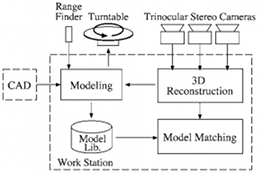
\includegraphics{figures/vvv}
\caption[Block diagram of VVV]{Block diagram of the ``VVV'' 3D vision robot system~\cite{sumi:2002}.}
\label{img:vvv}
\end{figure}

Another important contribution was given by Tomita \emph{et al.}~\cite{tomita:1998}: the Versatile 3D Vision system ``VVV'' can construct the 3D geometric data of any scene when two or more images are given, by using structural analysis and partial pattern matching. It can also recognize objects, although under the assumption that their geometric models are known. This is a relevant difference from our proposed approach, which, instead, is free of geometric models. A general user of VVV can make a task-oriented system whose ability is at least the same of a specialized robotic system (one that was built for a very specific action).

\bigskip

Within this chapter we will summarize the techniques that are related to the modules that compose our proposed architecture. Section~\ref{sec:segmentation} will outline the main image segmentation techniques existing in literature; Section~\ref{sec:stereopsis} will give a brief insight on stereo vision and 3D reconstruction; Section~\ref{sec:manipulation} will present the existing approaches for visual-based robot manipulator control; Section~\ref{sec:affordances} will introduce the object affordances learning tool, to improve manipulation performances.

%%%%%%%%%%%%%%%%
\section{Image Segmentation Techniques}
\label{sec:segmentation} \index{image segmentation}

The human eye is powerful because it is extremely \emph{versatile}: it can recognize objects nearly instantly, it can follow (track) their motion, recognize the mood of living beings from their facial expressions, decide when a circumstance is dangerous, compute the number and speed of objects, and more. It is because of this breadth of skills that the human eye is \emph{difficult to emulate}.

Recent \ac{CV} systems, on the other hand, are normally highly specialized; furthermore, they usually work well only under certain hypotheses. Some relevant fields of research inside \ac{CV} are tracking and image segmentation.

The purpose of image segmentation is to better organize the way we process a picture, by separating the interesting or relevant parts from those which are not useful for a given problem. Image segmentation, or simply ``segmentation''\index{segmentation|see{image segmentation}} for brevity, consists of dividing an image into two or more subset regions that cover it, according to a certain criterion, in order to simplify the representation and focus the attention on relevant parts of the image~\cite{foley}.

\begin{figure}
\centering
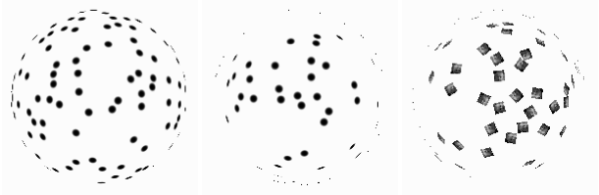
\includegraphics[scale=0.5]{figures/segm_3blobs}
\caption[Why segmentation is difficult]{Why segmentation is difficult: these are three surfaces whose image information can be organized into meaningful assemblies easily and successfully by the human eye, but it is not straightforward to do so for machines.}
%Picture: \cite{forsyth}.
\label{img:segment_3blobs}
\end{figure}

One of the major difficulties in object recognition problems is knowing \emph{which} pixels we have to recognize, and which to ignore~\cite{forsyth}. For example, it is difficult to tell whether a pixel lies on the surfaces in Fig.~\ref{img:segment_3blobs} simply by looking at the pixel. Specifically, it is difficult to tell whether a pixel lies on the three surfaces in the picture simply by looking at the pixel; the solution to the problem is to work with a \emph{compact representation} of the ``interesting'' image data that emphasize relevant properties. Segmentation is the process of obtaining such compact representation~\cite{shapiro_stockman}.

The goal in many tasks is for the regions to represent \emph{meaningful} areas of the image, such as crops, urban areas, and forests of a satellite image. Each of the resulting subsets contains those pixels of the image which satisfy a given condition: for instance, having the same colour, the same texture, or having rough edges. Furthermore, changing the representation of an image to something more meaningful means that it also becomes \emph{easier to analyze} and process.

Practical applications\index{image segmentation!applications} of image segmentation include:
\begin{itemize}
\item recognizing a face or any other trait that is \emph{salient} in a given situation;

\item traffic controlling systems;

\item medical imaging:
	\begin{itemize}
	\item[-] revealing, diagnosing and examining tumours;
	
	\item[-] studying other pathologies and anatomical structures;
		
	\item[-] measure the volume of tissues;
	
	\item[-] computer-guided surgery;
	\end{itemize}

\item locate objects in satellite images;

\item fingerprint recognition.
\end{itemize}

Traditionally~\cite[ch.~10]{shapiro_stockman}, segmentation has had two objectives:
\begin{enumerate}
\item to decompose the image into parts for further analysis;

\item to perform a change of representation.
\end{enumerate}

The importance of the first objective is straightforward to understand and is discussed thoroughly in texts like~\cite{foley, forsyth, shapiro_stockman, trucco_verri}. The second one, however, is more subtle: the pixels of an image must be organized into higher-level units that are either more meaningful or more efficient for further analysis, or both. A critical issue is whether or not segmentation can be performed for many different domains using bottom-up methods that do not use any special domain knowledge.

\bigskip

Since there is no general solution to the image segmentation\index{image segmentation} problem, several different approaches to implement segmentation have been proposed in literature, each having its advantages and drawbacks. A brief list of the most common techniques will now be given. Further down, the \ac{CAMSHIFT}\index{CAMSHIFT} algorithm, which belongs to the class of histogram-based\index{image segmentation!histogram-based} segmentation approaches (see~Section~\ref{sec:histo}) and is the technique adopted in this thesis, will be detailed.

%%%%%%%%%%%%%%%%
\subsection{Clustering Segmentation}
\index{image segmentation!clustering}

In pattern recognition, \emph{clustering} is the process of partitioning a set of pattern vectors into subsets called clusters~\cite{theodoridis}. Several types of clustering algorithms have been found useful in image segmentation. %These include classical clustering algorithms, simple histogram-based methods, Ohlander's recursive histogram-based technique, and more.

One way to look at the segmentation problem is thus to attempt to determine which components of a data set naturally ``belong together'' in a cluster. Generally, two approaches for clustering are considered in literature~\cite{forsyth}:

\begin{description}
\item[partitioning:] carving up a large data set according to some notion of the association between items inside the set, i.e., decomposing the set into pieces that are good with regards to a model. For example:
	\begin{itemize}
	\item[-] decomposing an image into regions that have coherent colour and texture inside them;
	
	\item[-] decomposing an image into extended blobs, consisting of regions that have coherent colour, texture and motion and look like limb segments;
	
	\item[-] decomposing a video sequence into shots---segments of video showing about the same scene from about the same viewpoint.
	\end{itemize}

\item[grouping:] starting from a set of distinct data items, collect sets of these items that make sense \emph{together} according to a model. Effects like occlusion mean that image components that belong to the same object are often separated. Examples of grouping include:
	\begin{itemize}
	\item[-] collecting together tokens that, when taken together, form a line;
	
	\item[-] collecting together tokens that seem to share a fundamental matrix.
	\end{itemize}
\end{description}

The key issue in clustering is to determine a suitable representation for the problem in hand.

\label{kmeans}
A famous clustering algorithm is $k$-Means\index{image segmentation!clustering!$k$-Means}, first described in~\cite{macqueen:1967}. Basic pseudocode is shown in Algorithm~\ref{algo:kmeans}. $k$-Means is an iterative technique to partition an image into $k$ clusters. The algorithm works by randomly selecting centroids, finding out which elements are closest to the centroid, then working out the mean of the points belonging to each centroid, which becomes the new centroid. Region membership is checked again, and the new centroids are computed again. This operation continues until there are no points that change their region membership.

\begin{algorithm}
\caption{Basic $k$-Means}
\label{algo:kmeans} \index{image segmentation!clustering!$k$-Means}
\begin{algorithmic}[1]
\STATE Place $k$ points into the space represented by the objects that are being clustered. These points represent initial group centroids.
\STATE Assign each object to the group that has the closest centroid.
\STATE When all objects have been assigned, recalculate the positions of the $k$ centroids. 
\STATE Repeat Steps 2 and 3 until the centroids no longer move. This produces a separation of the objects into groups from which the metric to be minimized can be calculated.
\end{algorithmic}
\end{algorithm}

While the $k$-Means algorithm is guaranteed to converge, it has a few drawbacks:
\begin{itemize}
\item it may occur that $k$-Means converges to a local, possibly not global, solution;

\item the algorithm is significantly sensitive to the initial randomly-selected cluster centres (to reduce this effect, one can execute $k$-Means multiple times, but this is costly);

\item basic $k$-Means relies on the assumption that the number of clusters $k$ is known in advance. Alternatives have been proposed to overcome this limitation of the initial setting, for example ``Intelligent $k$-Means''\index{image segmentation!clustering!Intelligent $k$-Means} by Mirkin~\cite[p.~93]{mirkin}.
\end{itemize}

% don't forget that EM is a variant of $k$-Means

%%%%%%%%%%%%%%%%
\subsection{Edge Detection Segmentation}
\label{sec:edge_det} \index{image segmentation!edge detection}

% [b]
\begin{figure}
\centering
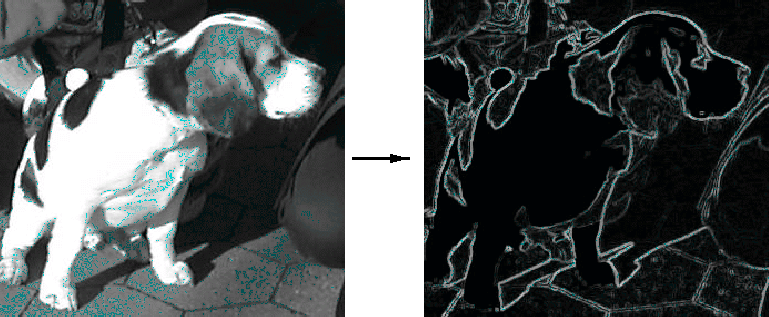
\includegraphics[scale=0.45]{figures/dog_edges}
\caption[Edge-based segmentation]{An example of edge-based segmentation, showing the computed edges of the left input image on the right.}
\label{img:dog_edges}
\end{figure}

\emph{Edge points}, or simply ``edges'', are pixels at or around which the image values undergo a sharp variation.

Edge detection techniques have been used as the base of several segmentation techniques, exploiting the tight relationship that exists between region boundaries and edges---the sharp adjustment in intensity at the region boundaries, as in Fig.~\ref{img:dog_edges}.

\begin{figure}
\centering
\subfloat[][A $325 \times 237$-pixel image, with scanline $i = 56$ (over the baby's forehead) highlighted.]
{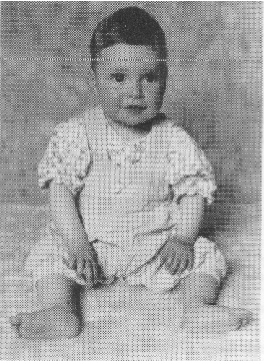
\includegraphics[width=.4\columnwidth]{figures/edge_baby} \label{fig:edge_baby} } \quad
% %necessary to prevent line break
\subfloat[][Intensity profile along the highlighted scanline.]
{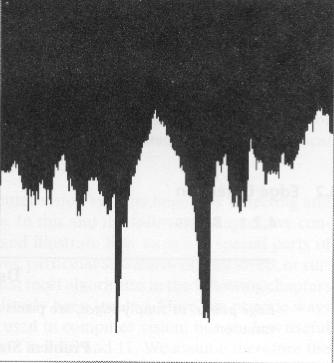
\includegraphics[width=.5\columnwidth]{figures/edge_baby_int} \label{fig:edge_baby_int} }

\caption[Edge detection and intensity profile]{An intensity image (left) and the intensity profile along a selected scanline (right). The main sharp variations correspond to significant contours.}
\label{fig:edge_det}
\end{figure}

The edge detection\index{image segmentation!edge detection} problem can be formulated like this: given an image that has been corrupted by acquisition noise, locate the edges most likely to be generated by scene elements (not by noise). Fig.~\ref{fig:edge_det} shows an example of edge detection computations.

Though, the edges identified by edge detection are often disconnected. To segment an object from an image, however, one needs closed region boundaries. Discontinuities are normally bridged if the distance between the two edges is within some predetermined threshold.

The Canny edge detection algorithm~\cite{canny:1986} \index{image segmentation!edge detection!Canny edge detection} is known as the optimal edge detector. It follows a list of three criteria with the aim of improving previous methods of edge detection:

\begin{description}
\item[good detection:] the algorithm should mark as many real edges in the image as possible. This is the first and most obvious principle, that of low error rate. It is important that edges occurring in images should not be missed and that there be no responses to non-edges.

\item[good localization:] the edges marked should be as close as possible to the edges in the real image. This second criterion suggests that the edge points should be well localized, in other words, that the distance between the edge pixels as found by the detector and the actual edge is to be at a minimum.

\item[minimal response:] a given edge in the image should only be marked once, and, where possible, image noise should not create false edges. The third criterion is thus to have only one response to a single edge; this was implemented because the first two criteria were not sufficient to completely eliminate the possibility of multiple responses to an edge.
\end{description}

To satisfy these requirements, the calculus of variations \index{calculus of variations} (a technique which finds the function which optimizes a given functional) is employed~\cite{canny:1986}. The optimal function in Canny's detector\index{image segmentation!edge detection!Canny edge detection} is described by the sum of four exponential terms, but can be approximated by the first derivative of a Gaussian. See Fig.~\ref{fig:canny} for an example.

\begin{figure}
\centering
\subfloat[][Input image: a colour photograph of a steam engine.]
{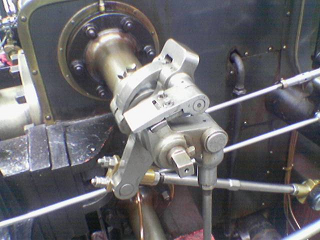
\includegraphics[width=.45\columnwidth]{figures/canny_valve_input} \label{fig:canny_valve_input} } \quad
%
\subfloat[][After having passed a $5 \times 5$ Gaussian mask across each pixel for noise reduction, the input image becomes slightly blurred.]
{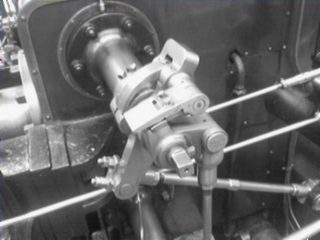
\includegraphics[width=.45\columnwidth]{figures/canny_valve_5pass} \label{fig:canny_valve_5pass} } \\
%
\subfloat[][Result of Canny edge detector.]
{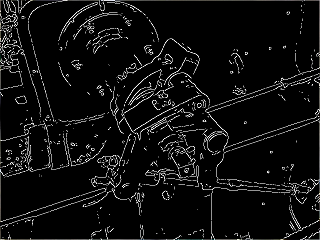
\includegraphics[width=.45\columnwidth]{figures/canny_valve_result} \label{fig:canny_valve_result} }
%
\caption[Canny edge detector]{Canny edge detector example.}
\label{fig:canny}
\end{figure}

%%%%%%%%%%%%%%%%
\subsection{Graph Partitioning Segmentation}
\index{image segmentation!graph partitioning}

Various algorithms exist in this class of methods, all of which model (groups of) pixels as vertices of a graph, while graph edges define the correlation or similarity among neighbouring pixels.

Popular graph partitioning segmentation techniques include: normalized cuts\index{image segmentation!graph partitioning!normalized cuts}, random walker, minimum mean cut, and minimum spanning tree-based algorithms.

Originally proposed by Shi and Malik~\cite{shi:1997}, the normalized cuts\index{image segmentation!graph partitioning!normalized cuts} method involves the modelling of the input image as a weighted, undirected graph. Each pixel is a node in the graph, and an edge is formed between every pair of pixels; the weight of an edge is a measure of the \emph{similarity} between the pixels.

The image is partitioned into disjoint sets (called ``segments''; see Fig.~\ref{img:norm_cuts}) by removing the edges that connect the segments. The optimal partitioning of the graph is the one that minimizes the weights of the edges that were removed (the ``cut''). The algorithm seeks to minimize the ``normalized cut''\index{image segmentation!graph partitioning!normalized cuts}, which is the ratio of the cut to all of the edges in the set.

\begin{figure}
\centering
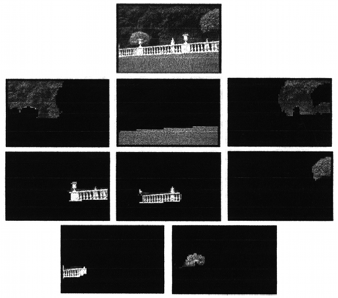
\includegraphics{figures/norm_cuts}
\caption[Graph partitioning segmentation: normalized cuts]{The image on top being segmented using the normalized cuts framework into the components shown below. The affinity measure used involved both intensity and texture. Thanks to having a texture measure, the railing shows as three reasonable coherent segments, which would not have happened with other approaches such as $k$-Means.}
\label{img:norm_cuts}
\end{figure}

%%%%%%%%%%%%%%%%
\subsection{Histogram-Based Segmentation}
\label{sec:histo} \index{image segmentation!histogram-based}

In this class of techniques, a histogram is computed from \emph{all} of the image pixels, taking into account colour or intensity values. Then, the peaks and valleys of such histogram are used to locate meaningful clusters in the image. By doing so, clusters are directly obtained after building the histogram.

See Fig.~\ref{img:colour_obj_tracking} for a generic scheme of these approaches. X, Y, and Area are relative to the colour probability distribution representing the tracked object (compare Section~\ref{sec:camshift_module}). Area is proportional to Z, i.e., the distance from the camera. Roll (inclination) is also tracked, as a fourth degree of freedom. For each video frame, the raw image is first converted to a colour probability distribution image via a colour histogram model of the colour being tracked (e.g., flesh for face tracking). The centre and size of the colour object are found via the \ac{CAMSHIFT}\index{CAMSHIFT} algorithm operating on the colour probability image. The current size and location of the tracked object are reported and used to set the size and location of the search window in the next video image. This process is iterated for continuous tracking.

Histogram-based segmentation\index{image segmentation!histogram-based} methods present an important advantage compared to other techniques: \emph{high efficiency}. Typically, these techniques require only one pass through the image pixels. For this reason, we will choose the \ac{CAMSHIFT}\index{CAMSHIFT}  algorithm, which belongs to this class, because we require a fast, simple, efficient tracker in our perceptual humanoid robotics framework.\index{perception}\index{humanoid robotics}

Building the histogram is a critical phase; as mentioned above, one can choose different types of measures like colour or intensity. This fact is important when envisioning a perceptual framework~\cite{bradski:1998}\index{PUI}, as is the case of our project and humanoid robotics.

\begin{figure}
\centering
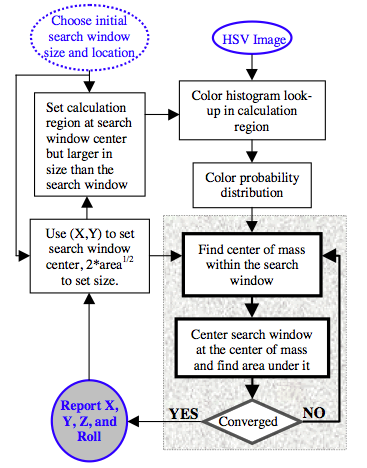
\includegraphics[scale=0.6]{figures/colour_obj_tracking}
\caption[Block diagram of object tracking]{Block diagram of histogram-based object tracking. The grey box is the Mean Shift\index{Mean Shift} algorithm.%
}
\label{img:colour_obj_tracking}
\end{figure}

A \ac{PUI} \index{PUI} is one in which a machine is given the ability to send and produce analogs of human senses, such as allowing computers to perceive\index{perception}\index{cognition} and produce localized sound and speech, giving robots a sense of touch and force feedback, or the ability to see.

% TODO: talk here about Mean Shift and CAMSHIFT?









%%%%%%%%%%%%%%%%
\subsection{Level Set Segmentation}
\label{sec:level_set} \index{image segmentation!level set}

In general, level set segmentation is a method for tracking the evolution of contours and surfaces. Originally proposed in~\cite{osher:1988}, this technique uses \ac{PSC}\index{PSC} schemes. The idea is to move surfaces under their curvature, propagating the surfaces towards the lowest potential of a cost function.

This framework has several advantages:
\begin{itemize}
\item level sets yield a useful representation of regions and their boundaries on the pixel grid without the need of complex (and costly) data structures. Therefore, optimization is simplified, as variational methods and standard numerics can be employed;

\item level sets can describe topological changes in the segmentation, i.e., parts of a region can split and merge;

\item it is possible to describe the image segmentation problem with a variational model, thus increasing flexibility (and permitting the introduction of additional features, shape knowledge, or joint motion estimation and segmentation).
\end{itemize}

\begin{figure}
\centering
\subfloat[][Input image.]
{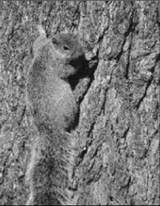
\includegraphics[width=.45\columnwidth]{figures/squirrel_ls1} \label{fig:squirrel_ls1} } \quad
% %necessary to prevent line break
\subfloat[][Level set segmentation.]
{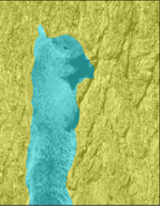
\includegraphics[width=.45\columnwidth]{figures/squirrel_ls2} \label{fig:squirrel_ls2} }
\caption[Level set segmentation]{Level set segmentation of a squirrel image: two regions have been detected.}
\label{fig:squirrel_ls}
\end{figure}

On the other hand, level set segmentation\index{image segmentation!level set} has a problem: a level set function is restricted to the separation of only two regions. Brox and Weickert~\cite{brox:2004} proposed a new formulation of the potential function to minimize, taking into account the number of regions, too.

\begin{figure}
\centering
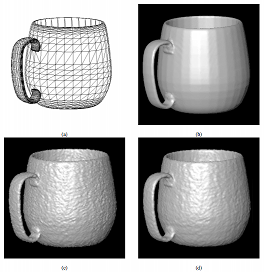
\includegraphics{figures/level_set_mug}
\caption[Level set based 3D reconstruction]{Level set based 3D reconstruction of a mug, using synthetic data generated from a 3D model~(a). Without noise, the reconstruction~(b) is limited only by the resolution of the model, $140 \times 140 \times 140$. With noise, the surface appears rough~(c). Including a prior improves the appearance of the reconstruction~(d).%
}
\label{img:level_set_mug}
\end{figure}

What is more, level set segmentation\index{image segmentation!level set} is well suited to generate 3D reconstructions\index{3D reconstruction} of objects~\cite{whitaker:1998}. See Fig.~\ref{img:level_set_mug} for a sample run of Whitaker's algorithm\index{image segmentation!level set!Whitaker's algorithm}. The strategy applied is as follows: construct a rather coarse volume that is the solution to a linear problem, i.e., the zero-level sets of a function, without the prior. This volume will serve as initialization for a level set model which moves towards the data given by range maps while undergoing a second-order flow to enforce the prior. After the rate of deformation slows to below some predefined threshold, the resolution is increased, the volume resampled, and the process repeated (in an attempt to avoid convergence to local minima).

Note that this last strategy employs predefined models of shapes: the approach has much to share with model-based segmentation methods, explained below.

%%%%%%%%%%%%%%%%
\subsection{Model-Based Segmentation}
\index{image segmentation!model-based}

Model-based segmentation approaches (or knowledge-based segmentation), commonly adopted in medical imaging\index{image segmentation!medical imaging}, rely on the assumption that structures of interest have a repetitive form of geometry.

State of the art methods in the literature for knowledge-based segmentation~\cite{freedman:2005} involve active shape and appearance models, active contours and deformable templates (see Fig.~\ref{img:model_based_prostate} for an example). Note that there is an intersection with level set segmentation methods\index{image segmentation!level set} (refer to Section~\ref{sec:level_set}).

One can seek a probabilistic model that explains the variation of the shape, for instance, of an organ and then, when segmenting an image, impose constraints using this model as a prior. Specifically, such a task involves:
\begin{enumerate}
\item registration\footnote{Registration fits models that are previously known; 3D reconstruction extracts models from images.}\index{registration} of the training examples to a common pose;

\item probabilistic representation of the variation of the registered samples; and

\item statistical inference between the model and the image.
\end{enumerate}

\begin{figure}
\centering
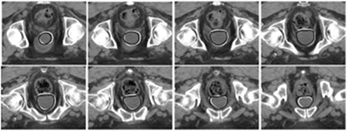
\includegraphics{figures/model_based_prostate}
\caption[Model based segmentation]{Model based segmentation results using a prostate model, to detect carcinoma cell masses. The white contour shows the result at convergence; the black contour shows the hand-drawn ground-truth contours supplied by a radiation oncologist.%
}
\label{img:model_based_prostate}
\end{figure}

So, these algorithms are based on matching probability distributions of photometric variables that incorporate learned shape and appearance models for the objects of interest. The main innovation is that there is no need to compute a pixel-wise correspondence between model and image. This allow for fast, principled methods.

%%%%%%%%%%%%%%%%
\subsection{Neural Networks Segmentation}
\index{image segmentation!neural networks}

Neural network image segmentation typically relies on processing \emph{small areas} of an image using an unsupervised neural network (a network where there is no external teacher affecting the classification phase) or a set of neural networks.

After such processing is completed, the decision-making mechanism marks the areas of an image accordingly to the category recognized by the neural network, as exemplified in Fig.~\ref{fig:nn_human_head}. A type of network well designed for these purposes~\cite{reyes:2000} is the Kohonen\index{Kohonen|see{\ac{SOM}}} \ac{SOM}\index{SOM}.

\begin{figure}
\centering
\subfloat[][Human head Magnetic Resonance input image.]
{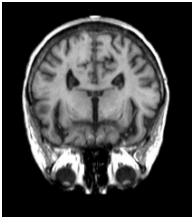
\includegraphics[width=.45\columnwidth]{figures/nn_human_head_input} \label{fig:nn_human_head_input} } \quad
%
\subfloat[][Neural Networks segmentation of MR image.]
{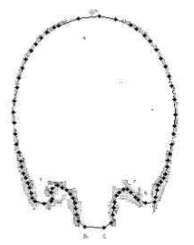
\includegraphics[width=.45\columnwidth]{figures/nn_human_head_segm} \label{fig:nn_human_head_segm} }
\caption{Neural Networks segmentation.}
\label{fig:nn_human_head}
\end{figure}

%%%%%%%%%%%%%%%%
\subsection{Region Growing Thresholding Segmentation}
\index{image segmentation!region growing}

Just like edge detection\index{image segmentation!edge detection} (see Section~\ref{sec:edge_det}) is implemented by quite different processes in photographs and range data, segmenting image into \emph{regions}\index{image segmentation!region growing}
 presents a similar situation.

Region growing is an approach to image segmentation in which neighbouring pixels are examined and added to a region class if no edges are detected~\cite{forsyth}. This process is iterated for each boundary pixel in the region. If adjacent regions are found, region-merging techniques are used in which weak edges are dissolved and strong edges are left intact.

This method offers several advantages over other techniques:
\begin{itemize}
\item unlike edge detection methods (such as gradient and Laplacian), the borders of regions found by region growing are thin --since one only adds pixels to the exterior of regions-- and connected;

\item the algorithm is stable with respect to noise: the resulting region will never contain too much of the background, as long as the parameters are defined correctly;

\item membership in a region can be based on multiple criteria, allowing us to take advantage of several image properties, such as low gradient or gray level intensity value, at once.
\end{itemize}

There are, however, disadvantages to region growing\index{image segmentation!region growing}. First and foremost, it is very \emph{expensive} computationally: it takes both serious computing power (processing power and memory usage) and a decent amount of time to implement and run the algorithms efficiently.

An example of region growing thresholding is~\cite{faugeras:1986}. This algorithm iteratively merges planar patches by maintaining a graph whose nodes are the patches and whose arcs (edges) are associated with their common boundary link adjacent patches. Each arc is assigned a cost, corresponding to the average error between the points of the two patches and the plane best fitting these points. The best arc is always selected, and the corresponding patches are merged. Note that the remaining arcs associated with these patches must be deleted while new arcs linking the new patch to its neighbors are introduced. The situation is illustrated by Fig.~\ref{img:region_growing}.

\begin{figure}
\centering
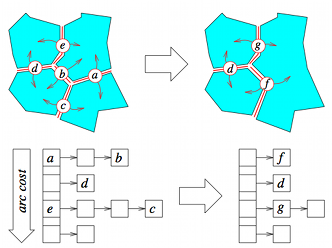
\includegraphics{figures/region_growing}
\caption[Region growing]{One iteration of the region growing process during which the two patches incident on the minimum-cost arc labelled $a$ are merged. The heap shown in the bottom part of the figure is updated as well (which bears a considerable computational cost): the arcs $a, b, c$ and $e$ are deleted, while two new arcs $f$ and $g$ are created and inserted in the heap.}
\label{img:region_growing}
\end{figure}

% this is a variant of the seeded region growing technique ->  requires the input of a number of seeds, either individual pixels or regions, which will control the formation of regions into which the image will be segmented
%One variant of this technique, proposed by Shapiro~\cite{shapiro_stockman}, is based on pixel intensities. The mean and scatter of the region and the intensity of the candidate pixel is used to compute a test statistic. If the test statistic is sufficiently small, the pixel is added to the region, and the region's mean and scatter are recomputed; otherwise, the pixel is rejected and it is used to form a new region.

%%%%%%%%%%%%%%%%
\subsection{Scale-Space Segmentation}
\index{image segmentation!scale-space}

Scale-space segmentation, also known as multi-scale segmentation, is based on the computation of image descriptors at multiple scales of smoothing. It is a general technique used for signal and image segmentation (see Fig.~\ref{img:scale-space_repr} and Fig.~\ref{img:scale-space_segm_ex}).

The main type of scale-space\index{image segmentation!scale-space} is the linear (Gaussian) scale-space, which has wide applicability as well as the attractive property of being possible to derive from a small set of scale-space axioms. The corresponding scale-space framework encompasses a theory for Gaussian derivative operators, which can be used as a basis for expressing a large class of visual operations for computerized systems that process visual information. This framework also allows visual operations to be made scale-invariant, which is necessary for dealing with the size variations that may occur in image data, because real-world objects may be of different sizes and in addition the distance between the object and the camera may be unknown and may vary depending on the circumstances.

For a two-dimensional image $f(x,y)$, its linear (Gaussian) scale-space \emph{representation} is a family of derived signals $L(x,y; t)$ defined by the convolution of $f(x,y)$ with the Gaussian kernel
\begin{equation}
g_t(x,y) = \frac{1}{2\pi t}e^{-(x^2 + y^2)/2t}
\end{equation}
such that
\begin{equation}
L(x,y; t) = (g_t * f)(x,y),
\end{equation}
where the semicolon in the argument of $L$ implies that the convolution is performed only over the variables $x,y$, while the scale parameter $t$ after the semicolon just indicates which scale level is being defined. This definition of $L$ works for a continuum of scales , but typically only a finite discrete set of levels in the scale-space representation would be considered.

\begin{figure}
\centering
\subfloat[][$t = 0$, corresponding to the original image $f$.]
{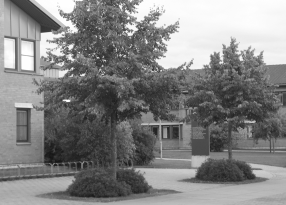
\includegraphics[width=.45\columnwidth]{figures/scale-space0} \label{img:scale-space0} } \quad
%
\subfloat[][$t = 1$.]
{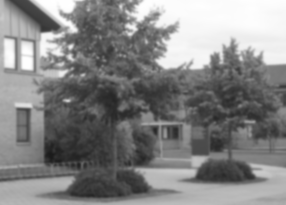
\includegraphics[width=.45\columnwidth]{figures/scale-space1} \label{img:scale-space1} } \\
\subfloat[][$t = 4$.]
{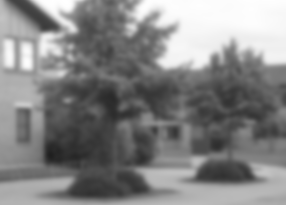
\includegraphics[width=.45\columnwidth]{figures/scale-space4} \label{img:scale-space4} } \quad
%
\subfloat[][$t = 16$.]
{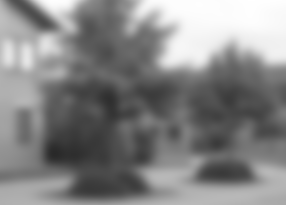
\includegraphics[width=.45\columnwidth]{figures/scale-space16} \label{img:scale-space16} }
%
\caption[Space-scale representation]{Space-scale representation $L(x,y; t)$ for various $t$ scales. As the parameter $t$ increases above $0$, $L$ is the result of smoothing $f$ with a larger and larger filter.}
\label{img:scale-space_repr}
\end{figure}

In Fig.~\ref{img:scale-space_dendro}, each ``x'' identifies the position of an extremum of the first derivative of one of 15 smoothed versions of the signal (red for maxima, blue for minima). Each ``+'' identifies the position that the extremum tracks back to at the finest scale. The signal features that persist to the highest scale (smoothest version) are evident as the tall structures that correspond to the major segment boundaries in the figure above.

\begin{figure}
\centering
\subfloat[][A signal (black), various multi-scale smoothed versions of it (red) and some segment averages (blue).]
{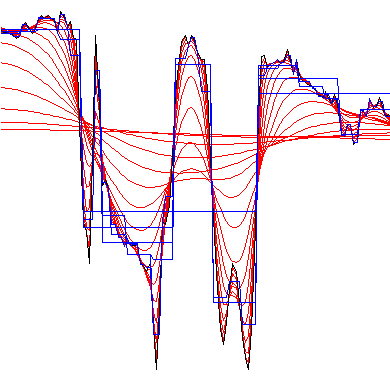
\includegraphics[width=.80\columnwidth]{figures/scale-space_segm} \label{img:scale-space_segm} } \\
%
\subfloat[][Dendrogram resulting from the segmentation in Fig.~\ref{img:scale-space_segm}.]
{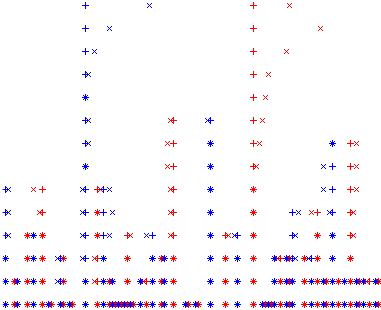
\includegraphics[width=.80\columnwidth]{figures/scale-space_dendro} \label{img:scale-space_dendro} }
\caption[Space-scale segmentation]{Space-scale segmentation example.}
\label{img:scale-space_segm_ex}
\end{figure}

%%%%%%%%%%%%%%%%
\subsection{Semi-Automatic Livewire Segmentation}
\index{image segmentation!semi-automatic}
\index{image segmentation!Livewire|see{image segmentation!semi-automatic}}

In this segmentation method, the user outlines the \ac{ROI} with mouse clicks, then an algorithm is applied so that the path that best fits the edge of the image is shown. It is based on the lowest cost path algorithm by Dijkstra\index{Dijkstra's algorithm}. 

The user sets the starting point clicking on an image pixel. Then, as he starts to move the mouse over other points, the smallest cost path is drawn from the starting point to the pixel where the mouse is over, changing itself if the user moves the mouse. If the user wants to choose the path that is being displayed, he will simply click the image again.

\begin{figure}
\centering
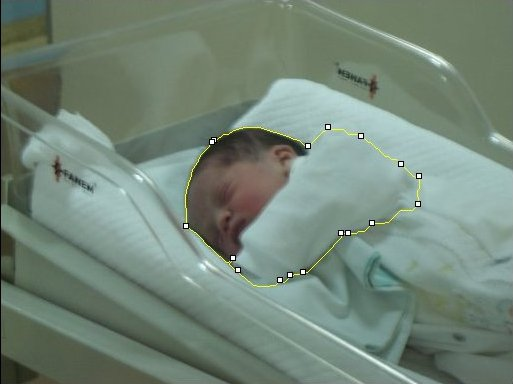
\includegraphics[scale=0.8]{figures/livewire_baby}
\caption[Semi-automatic Livewire segmentation]{Example run of a semi-automatic Livewire technique applied on a picture.}
\label{img:livewire_baby}
\end{figure}

One can easily see in Fig.~\ref{img:livewire_baby} that the places where the user clicked to outline the desired \ac{ROI} are marked with a small square. It is also easy to see that Livewire\index{image segmentation!semi-automatic} has snapped on the image borders.

% related technique: Intelligent Scissors

%%%%%%%%%%%%
%%%%%%%%%%%%
\section{Stereopsis}
\label{sec:stereopsis}
\index{stereopsis} \index{stereo vision|see{stereopsis}}

Since a considerable portion of this thesis work deals with how a humanoid robot can perceive object positions and orientations in 3D space by using a binocular head (see Section~\ref{sec:3d_recon_approach}), some introductory theoretical background is first due.

Stereopsis, also known as stereo vision or simply ``stereo'', allows two-dimensional images to be interpreted in terms of 3D scene structure and distance~\cite{trucco_verri}.

Humans have an uncanny ability to perceive and analyze the structure of the 3D world from visual input, operating effortlessly and with little or no idea of what the mechanisms of visual perception are.

Depending on the nature of the features we wish to observe (2D or 3D, points or lines on the surface of the object, etc.), different formulations and algorithms come into play. However, the underlying mathematics has much in common: all the different cases can be formulated in such a way that they require solutions of simultaneous transcendental, polynomial, or linear equations in multiple variables which represent the structure of the object and its 3D motion as characterized by rotation and translation.

\begin{figure}
\centering
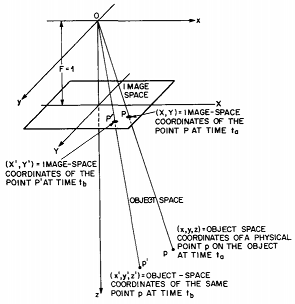
\includegraphics{figures/perspective_geom}
\caption[Perspective geometry for imaging]{Basic perspective geometry for imaging. Lower case letters refer to coordinates in the object space, upper case letters to coordinates on the image plane. Focal length (denoted here with $F$) is assumed to be $1$.}
\label{img:perspective_geom}
\end{figure}

In particular, what is inferred is a sensation of depth from the two slightly different projections of the world onto the retinas of the two eyes. The differences in the two retinal images are called horizontal disparity\index{horizontal disparity}, retinal disparity\index{retinal disparity|see{horizontal disparity}}, or binocular disparity\index{binocular disparity|see{horizontal disparity}}. The differences arise from the eyes' different positions in the head.

Stereo vision involves two processes:
\begin{itemize}
\item the binocular fusion of features observed by the two eyes;

\item the actual reconstruction of the features observed in the world.
\end{itemize}

They can be translated into two problems:
\begin{description}
\item[correspondence:]\index{correspondence} which parts of the left and right images are projections of the same scene element?

\item[reconstruction:]\index{3D reconstruction} given a number of corresponding parts of the left and right image, and possibly information on the geometry of the stereo system, what can we say about the 3D location and structure of the observed objects?
\end{description}

The correspondence problem is out of the scope of this project. In our proposed approach in Section~\ref{sec:3d_recon_approach}, we will focus on 3D reconstruction.

%%%%%%%%%%%%
%%%%%%%%%%%%
\section{Object Manipulation with Visual Servoing}\index{manipulation}
\label{sec:manipulation}

% which?
Existing visual-based robot control approaches~\cite{chaumette:visual1, chaumette:visual2, hutchinson:1996}, summarized below, solve the issue of representing a gripper--object relationship by handling \emph{models} of gripper and object in memory. This approach, while accurate and powerful, presents two drawbacks:
\begin{itemize}
\item the object model may be poor; besides, in several circumstances it may not be available at all (as addressed by Malis and Chaumette~\cite{malis:2002} or by Dufournaud \emph{et al.}~\cite{dufournaud:1998});

\item computational cost is high due to the manipulation program having to memorize and compute comparison operations to such models.
\end{itemize}

Visual Servoing~\cite{corke}\index{Visual Servoing} is a multi-disciplinary approach to the control of robots based on visual perception, involving the use of cameras to control the position of the robot relative to the environment as required by the task. This technique uses visual feedback information extracted from a vision sensor, to control the motion of robots. This discipline spans \ac{CV}, robotics, control, and real-time systems.

The task in Visual Servoing is to control the pose (3D position and orientation) of a robot's end-effector, using visual information (features) extracted from images.

Visual Servoing methods are commonly classified as image-based or position-based\footnote{Some ``hybrid approaches'' have also been proposed: 2-1/2-D Servoing, Motion Partition Based Servoing, and Partitioned DOF Based Servoing.}, depending on whether image features or the camera position define the signal error in the feedback loop of the control law.

\subsection{Image-Based Visual Servoing}
\index{Visual Servoing!Image-Based Visual Servoing}

\ac{IBVS} is a feature-based technique, meaning that it employs features that have been extracted from the image to directly provide a command to the robot (without any computation by the robot controller). Typically for \ac{IBVS}, all the information extracted from the image features and used in control, occurs in a 2D space. In most cases this coincides with the image coordinates' space. Despite this 2D information, because of which the approach is also known as ``2D servoing control'', the robot still has the capability to move in 3D.

\ac{IBVS} involves the estimation of the robot's velocity screw, $\dot{\mathbf{q}}$, so as to move the image plane features, ${\mathbf{f}}^c$, to a set of desired locations, ${\mathbf{f}}^*$~\cite{malis:2002}. \ac{IBVS} requires the computation of the \emph{image Jacobian} (or \emph{interaction matrix}). The image Jacobian represents the differential relationships between the scene frame and the camera frame (where either the scene or the camera frame is attached to the robot):
%
\begin{equation}
\mathbf{J}(\mathbf{q}) =
	\begin{bmatrix}
	\frac{\partial \mathbf{f}}{\partial \mathbf{q}}
	\end{bmatrix} =
	\begin{bmatrix}
	\frac{\partial f_1(\mathbf{q})}{\partial q_1} & \dots & \frac{\partial f_1(\mathbf{q})}{\partial q_m} \\
	\vdots & \ddots & \vdots \\
	\frac{\partial f_k(\mathbf{q})}{\partial q_1} & \dots & \frac{\partial f_k(\mathbf{q})}{\partial q_m}
	\end{bmatrix}
\end{equation}
%
where $\mathbf{q}$ represents the coordinates of the end-effector in some parameterization of the task space $\mathcal{T}$, $\mathbf{f} = [f_1, f_2, \dots, f_k]$ represents a vector of image features, $m$ is the cardinality of the task space $\mathcal{T}$, and $k$ is the number of image features.

\subsection{Position-Based Visual Servoing}
\index{Visual Servoing!Position-Based Visual Servoing}

\ac{PBVS} is traditionally a model-based technique. The pose of the object of interest is estimated with respect to the camera frame, then a command is issued to the robot controller, which in turn controls the robot. In this case, the image features are extracted as well, like in \ac{IBVS}, though the feature information is used to estimate the 3D object pose information in Cartesian space.

\begin{figure}
\centering
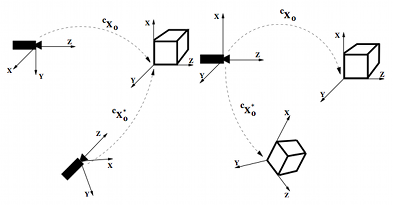
\includegraphics[scale=0.9]{figures/pbvs_examples}
\caption[Examples of \ac{PBVS}]{Two examples of \ac{PBVS} control. Left: eye-in-hand camera configuration, where the camera/robot is servoed from $\leftidx{^c}{\mathbf{x}}_0$ (current pose) to $\leftidx{^c}{\mathbf{x}}_0^*$ (desired pose). Right: a monocular, standalone camera system used to servo a robot-held object from its current to the desired pose.} 
\label{img:pbvs_examples}
\end{figure}

\ac{PBVS} is usually referred to as ``3D servoing control'', since image measurements are used to determine the pose of the target with respect to the camera and some common world frame. The error between the current and the desired pose of the target is defined in the task (Cartesian) space of the robot; hence, the error is a function of pose parameters, $\mathbf{e}(\mathbf{x})$. Fig~\ref{img:pbvs_examples} shows possible example tasks of \ac{PBVS}.

Fig~\ref{img:pbvs_block_diagram} illustrates the general working scheme of \ac{PBVS}, where the difference in pose between the desired and the current pose represents an \emph{error} which is then used to estimate the velocity screw for the robot, $\dot{\mathbf{q}} = [ \mathbf{V}; \mathbf{\Omega} ]^T$, in order to minimize that error.

\begin{figure}
\centering
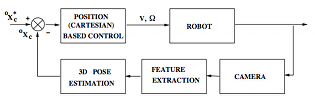
\includegraphics{figures/pbvs_block_diagram}
\caption[Block diagram of \ac{PBVS}]{Block diagram of \ac{PBVS}~\cite{hutchinson:1996}. The estimated pose of the target, $\leftidx{^c}{\mathbf{x}}_0$, is compared to the desired reference pose, $\leftidx{^c}{\mathbf{x}}_0^*$. This is then used to estimate the velocity screw, $\dot{\mathbf{q}} = [ \mathbf{V}; \mathbf{\Omega} ]^T$, for the robot so to minimize the error.}
\label{img:pbvs_block_diagram}
\end{figure}

%%%%%%%%%%%%
%%%%%%%%%%%%
\section{Object Affordances}
\label{sec:affordances}\index{object affordances}

Object affordances, or simply ``affordances'' for brevity, are a way to encode the relationships among actions, objects and resulting effects~\cite{montesano:2008}.

\begin{figure}
\centering
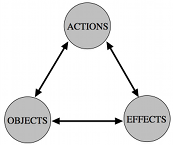
\includegraphics{figures/affordances}
\caption[Object affordances]{Object affordances represent the relationships that take place among actions (A), objects (O) and effects (E).}
\label{img:affordances}
\end{figure}

The general tool adopted to capture the dependencies in affordances (see Fig.~\ref{img:affordances}) is that of Bayesian networks\index{Bayesian networks}. Affordances make it possible to infer causality relationships by taking advantage of the intervention of a robot and the temporal ordering of events. Table~\ref{tab:affordances} lists the basic purposes of affordances.

\begin{table}
\caption[Purposes of object affordances]{Object affordances can be used for different purposes: to predict the outcome of an action, to plan the necessary actions to achieve a goal, or to recognize objects/actions.}
\label{tab:affordances}
\centering
\medskip
\begin{tabular}{*{3}{l}}
\toprule
input & output & function \\
\otoprule
$(O,A)$ & $E$ & predict effect \\
\midrule
$(O,E)$ & $A$ & action recognition and planning \\
\midrule
$(A,E)$ & $O$ & object recognition and selection \\
\bottomrule
\end{tabular}
\end{table}

Contrary to similar approaches, in the affordances framework the dependencies shown in Fig.~\ref{img:affordances} are \emph{not} known in advance (in which case we would learn a mapping between paris of actions and objects, or use supervised learning). Not assuming any prior knowledge on these dependencies, with affordances we try to infer the graph of the network directly from the exteroceptive and proprioceptive measurements. In addition, the affordances model allows the robot to tune the free parameters of the controllers.

This framework combines well with a developmental architecture whereby the robot incrementally develops its skills. In this sense, affordances can be seen as a bridge between
\begin{itemize}
\item sensory--motor coordination, and

\item world understanding and imitation.
\end{itemize}

Results on the learning and usefulness of object affordances for robots that use monocular vision (one camera only) are discussed in~\cite{montesano:2008}. With the (future) work of this thesis we intend to combine affordances with information obtained from stereo vision.

%%%%%%%%
% my approach
%%%%%%%%

%!TEX encoding = UTF-8 

\chapter{Robot Platform and Software Setup}
\label{chap:robot_platform}

\begin{figure}
\centering
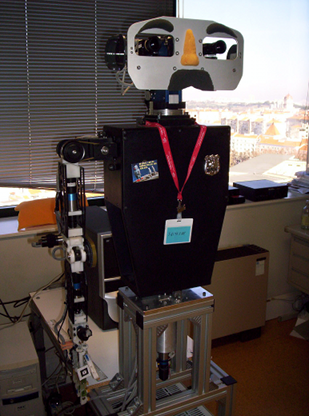
\includegraphics{figures/balta_relaxed}
\caption[Baltazar humanoid robot in relax position]{Baltazar humanoid robot in relax position.}
\label{img:balta_relaxed}
\end{figure}

In 2004, Computer and Robot Vision Laboratory~\cite{link:vislab} at IST in Lisbon developed a humanoid robot platform, ``Baltazar''~\cite{lopes:2004}\index{Baltazar}, which was used for this work. Baltazar, shown in Fig.~\ref{img:balta_relaxed}, is an anthropomorphic torso that features a binocular head as well as an arm and a hand. It was built as a system that mimics human arm-hand kinematics as closely as possible, despite the relatively simple design.

Baltazar is well suited (and was designed) for research in imitation\index{imitation}, skill transfer and visuomotor coordination. The design of Baltazar was driven by these constraints:
\begin{itemize}
\item the robot should resemble a human torso;

\item the robot kinematics should be able to perform human-like movements and gestures, as well as to allow a natural interaction with objects during grasping;

\item payload should be at least 500 g (including the hand);

\item force detection should be possible;

\item the robot should be easy to maintain and be low cost (it contains regular DC motors with reduced backlash and off-the-shelf mechanical parts).
\end{itemize}

In this section we will summarize mechanical and kinematic details of Baltazar, its sensors and technology. More details (such as the design of the 11-\ac{DOF} hand of Baltazar, not actually used in this thesis work as we focus on grasping \emph{preparation}) can be found in~\cite[p.~113]{lopes:phd}.

A software library used to develop programs for Baltazar, called \ac{YARP}, is used extensively in the whole \ac{RobotCub} developers community and in the implementation of this thesis, therefore \ac{YARP} and its middleware mechanisms will also be described; other secondary software tools that we used will be cited.

%%%%%%%%%%%%%%%%%%%%%%
%%%%%%%%%%%%%%%%%%%%%%
\section{Kinematic Description of Baltazar}

Robot kinematics studies the \emph{motion} of robots, thus taking into account the positions, velocities and accelerations of robot links, but without regard to the forces that actually cause the motion (whose study belongs to robot dynamics): robot kinematics uses just geometrical constraints. The kinematics of manipulators involves the study of the geometric- and time-based properties of motion, in particular how the various links move with respect to one another and with time.

The vast majority of robots belong to the \emph{serial} link manipulator class, which means that it comprises a set of bodies called \emph{links} in a chain, connected by \emph{joints}\footnote{To be more accurate, parallel link and serial/parallel hybrid structures are theoretically possible, although they are not common.}. Each joint has one \ac{DOF}, either translational or rotational; for example, the anthropomorphic arm used for the work of this thesis has 6 rotational \acp{DOF}.

For a manipulator with $n$ joints numbered from $1$ to $n$, there are $n+1$ links, numbered from $0$ to $n$. Link $0$ is the base of the manipulator, while link $n$ carries the end-effector. Joint $i$ connects links $i$ and $i-1$.

% ?
The kinematic model of a robot expresses how its several components move among themselves, achieving a transformation between different configuration spaces. The ``spaces'' mentioned here are the ones of the Cartesian geometric world workspace, as opposed to less-intuitive spaces that are directly associated with the robot's joint parameters, which are usually~\cite{craig, sciavicco_siciliano} denoted as a vector $\mathbf{q}$.

The following types of kinematics approaches are commonly studied in robotics:
\begin{description}
\item[forward kinematics] computes the position of a point in space (typically, that of the end-effector), given the values of the joint parameters (lengths and angles);

\item[inverse kinematics] computes all the joint parameters, given a point in space that the end-effector must lie on;

\item[forward velocity kinematics] (or forward differential kinematics) computes the velocity of a point in space, given the derivatives of the joint parameters;

\item[inverse velocity kinematics] (or inverse differential kinematics) computes the derivatives, i.e., velocities of joint parameters, given spatial velocities.
\end{description}

Forward kinematics (also known as direct kinematics) is the problem of transforming the joint positions of a robot to its end-effector pose. In other words, it is the computation of the position and orientation of a robot's end-effector as a function of its joint angles. For example, given a serial chain of $n$ links and letting $\theta_i$ be the angle of link $i$, then the reference frame of link $n$ relative to link $0$ is
\[
\leftidx{^0} {\mathbf{T}}_n = \prod_{i=1}^n  \leftidx{^{i-1}}{\mathbf{T}}_i (\theta_i)
\]
where $\leftidx{^{i-1}}{\mathbf{T}}_i(\theta_i)$ is the transformation matrix from the frame of link $i$ to that of link $i-1$.


%%%%%%%%%%%%%%%
\subsection{Kinematic Notation}
\index{Denavit-Hartenberg (DH)}
\index{Denavit-Hartenberg (DH)!SDH} \index{Denavit-Hartenberg (DH)!MDH}

\begin{figure}
\centering
\subfloat[][\acl{SDH} (\acs{SDH}) convention.]
{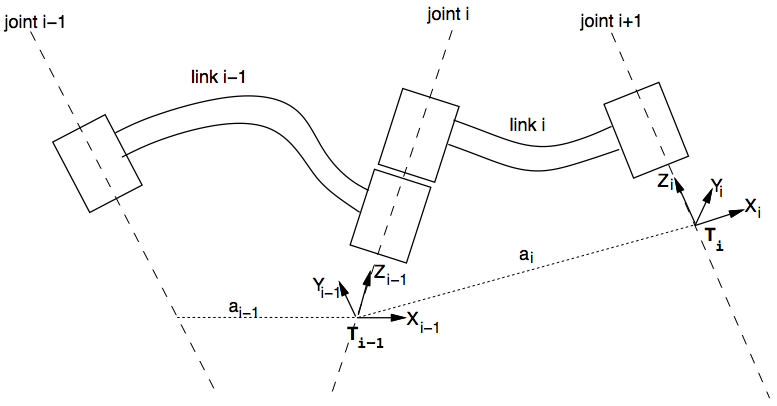
\includegraphics[width=.45\columnwidth]{figures/standard_dh} } \quad
% %necessary to prevent line break
\subfloat[][\acl{MDH} (\acs{MDH}) convention.]
{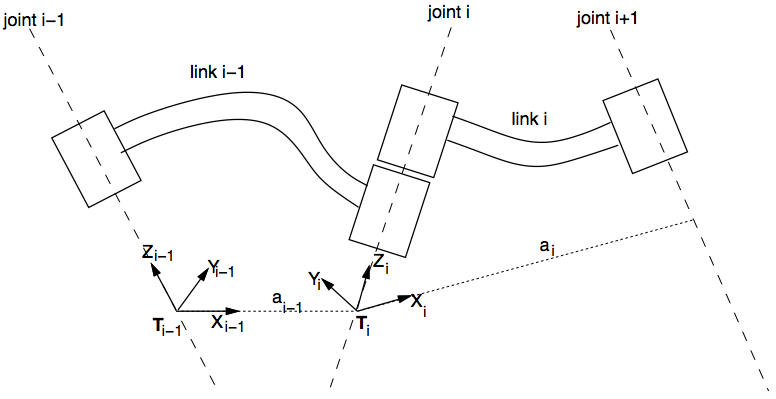
\includegraphics[width=.45\columnwidth]{figures/modified_dh} }

\caption[Different forms of \acs{DH} notation]{Different forms of \ac{DH} notation. Note: $a_i$ always indicates the length of link $i$, but the displacement it represents is between the origins of frame $i$ and frame $i+1$ in the standard form, between frames $i-1$ and $i$ in the modified form.

%Picture: Robotics Toolbox for MATLAB.
}
\label{fig:dh}
\end{figure}

A word of advice on the study and notation of kinematics: in robotics literature, at least two related but different conventions to model serial manipulator kinematics go by the name \ac{DH}, however they actually vary in a few details related to the assignment of reference frames to the rigid bodies (links) of robots.

These differences among \ac{DH} parameterizations are rarely acknowledged (with the exception of~\cite{corke:1996}). Typically, an author chooses one of the existing \ac{DH} notations, writes down ``this is the Denavit-Hartenberg convention'' then sticks to it from that moment on. One should, however, pay attention to which \ac{DH} formulation is being used and understand it.

Two different methodologies, shown in Fig.~\ref{fig:dh}, have been established to assign coordinate frames:
\begin{enumerate}
\item \ac{SDH} form, also known as ``unmodified'' \ac{DH} convention: frame $i$ has its origin along the axis of joint $i+1$.

\item \ac{MDH} form: frame $i$ has its origin along the axis of joint $i$.
\end{enumerate}

\ac{MDH} is commonly used in the literature on manipulator mechanics, and the (forward and inverse) kinematics approaches for Baltazar that exist so far, have in fact followed the \ac{MDH} form. However, further on we will see cases where it is practical to make a change of representation to \ac{SDH} to model the arm of Baltazar by the means of publicly-available robotics simulation tools.

The difference between \ac{SDH} and \ac{MDH} is the following\marginpar{Difference between \ac{SDH} and \ac{MDH}.}. In \ac{SDH}, we position the origin of frame $i$ along the axis of joint $i+1$. With \ac{MDH}, instead, frame $i$ has its origin along the axis of joint $i$.

A point to stress is that the choices of the various reference frames to assign (with \acs{SDH} or with \acs{MDH}) are \emph{not unique}, even under the constraints that need to be enforced among consecutive links. For example, the origin of the first reference frame $O_0$ can be arbitrarily positioned anywhere on the first joint axis. Thus, it is possible to derive different, equally valid, coordinate frame assignments for the links of a given robot. On the other hand, the final matrix that transforms from the base to the end effector, $\leftidx{^n}{\mathbf{T}}_0$, must be the same---regardless of the intermediate frame assignments.

For a detailed description of \ac{DH} conventions and the meaning of the four parameters ($a$: link length; $\alpha$: link twist; $d$: link offset; $\theta$: joint angle) refer, for example, to:
\begin{itemize}
\item \cite{spong}, which explains \ac{SDH} thoroughly; Chapter~3 is publicly available\footnote{\url{http://www.cs.duke.edu/brd/Teaching/Bio/asmb/current/Papers/chap3-forward-kinematics.pdf}};

\item \cite{craig} for \ac{MDH}; or

\item \cite{corke:1996} (both parameterizations).
\end{itemize}



%\subsubsection{\ac{SDH} link transform}

If we use the \ac{SDH} representation, the following $4 \times 4$ homogeneous transformation matrix
%
\begin{equation}
\label{eq:sdh_transf}
\leftidx{^{i-1}}{\mathbf{A}}_i = 
\begin{bmatrix}
\cos\theta_i & -\sin\theta_i \cos\alpha_i & \sin\theta_i \sin\alpha_i & a_i \cos\theta_i \\
\sin\theta_i & \cos\theta_i \cos\alpha_i & -\cos\theta_i \sin\alpha_i & a_i \sin\theta_i \\
0 & \sin\alpha_i & \cos\alpha_i & d_i \\
0 & 0 & 0 & 1
\end{bmatrix}
\end{equation}
%
represents each link's coordinate frame with respect to the previous link's coordinate system, i.e.,
\begin{equation}\label{eq:transf}
\leftidx{^0}{\mathbf{T}}_i = \leftidx{^0}{\mathbf{T}}_{i-1} \quad \leftidx{^{i-1}}{\mathbf{A}}_i
\end{equation}
where $\leftidx{^0}{\mathbf{T}}_i$ is the homogeneous transformation describing the pose (position and orientation) of coordinate frame $i$ with respect to the world coordinate system $0$.

%\subsubsection{\ac{MDH} link transform}

With \ac{MDH}, Eq.~\ref{eq:transf} still holds, however the homogeneous transformation matrix assumes the following form (instead of Eq.~\ref{eq:sdh_transf}):
%
\begin{equation}\label{eq:mdh_transf}
\leftidx{^{i-1}}{\mathbf{A}}_i = 
\begin{bmatrix}
\cos\theta_i & -\sin\theta_i & 0 & a_{i-1} \\
\sin\theta_i \cos\alpha_{i-1} & \cos\theta_i \cos\alpha_{i-1} & -\sin\alpha_{i-1} & d_i \sin\alpha_{i-1} \\
\sin\theta_i \sin\alpha_{i-1} & \cos\theta_i \sin\alpha_{i-1} & \cos\alpha_{i-1} & d_i \cos\alpha_{i-1} \\
0 & 0 & 0 & 1
\end{bmatrix}
\end{equation}




%%%%%%%%%%%%%%%
\subsection{Head Structure}
\label{sec:balta_head} \index{Baltazar!head}

\begin{figure}
\centering
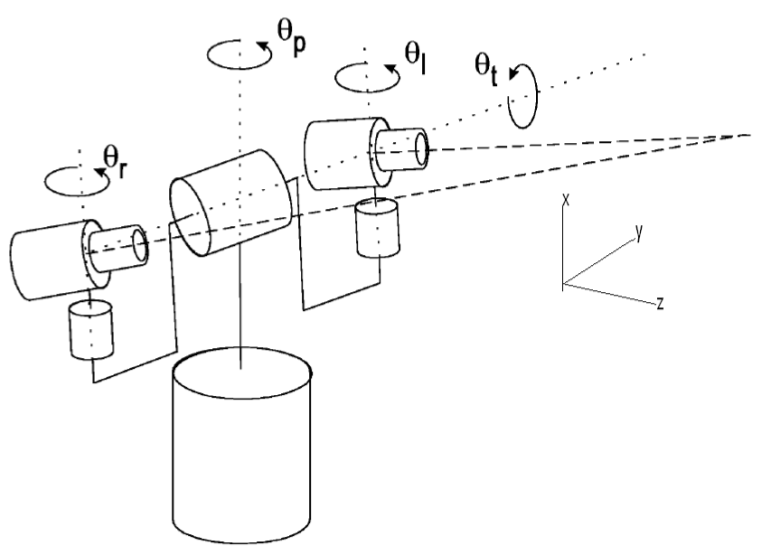
\includegraphics[scale=0.4]{figures/balta_head_scheme}
\caption[Scheme of Baltazar robotic head]{Scheme of Baltazar robotic head, code-named ``Medusa''~\cite{bernardino:1999}. The meaning of the four joint angles $\theta_l, \theta_r, \theta_p$ and $\theta_t$ is explained in Table~\ref{tab:balta_head_joints}.}
\label{img:balta_head_scheme}
\end{figure}

\begin{table}
\caption[Joint angles of Baltazar robotic head]{Joint angles of Baltazar robotic head.}
\label{tab:balta_head_joints}
\centering
\medskip
\begin{tabular}{*{2}{l}} % table with 2 left-aligned columns
\toprule
angle & description \\
\otoprule
$\theta_l$ & left eye camera vergence \\
\midrule
$\theta_r$ & right eye camera vergence \\
\midrule
$\theta_p$ & pan (neck rotation) \\
\midrule
$\theta_t$ & tilt (head rotation) \\
\bottomrule
\end{tabular}
\end{table}

The mechanical and geometrical structure of the robotic head used for this thesis work can be seen in Fig.~\ref{img:balta_head_scheme}, which shows the four \acp{DOF} of the head, all of which are rotational: neck rotation (pan), head elevation (tilt), left eye vergence, and right eye vergence.

\begin{figure}
\centering
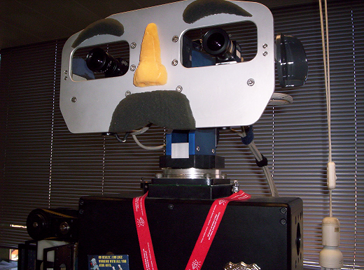
\includegraphics{figures/balta_head_real}
\caption[Real Baltazar robotic head]{Real Baltazar robotic head.}
\label{img:balta_head_real}
\end{figure}

A view of the real Baltazar robotic head, along with its two cameras, can be seen in Fig.~\ref{img:balta_head_real}.

Manual adjustments can be made to align the vergence and elevation axes of rotation with the optical centres of the cameras. Inter-ocular distance (baseline) can also be modified. \ac{MDH} parameters of the head are displayed in Table~\ref{tab:balta_head_mdh}.

\begin{table}
\caption[\acs{MDH} parameters of Baltazar binocular head]{A possible \ac{MDH} parameterization of the left eye of the binocular head of Baltazar, taken from~\cite{lopes:2004}. $B$ is the baseline distance between the two eyes.}
\label{tab:balta_head_mdh}
\centering
\medskip
\begin{tabular}{*{5}{l}} % table with 5 left-aligned columns
\toprule
Joint $i$ & $a_{i-1}$ [cm] & $d_i$ [cm]& $\alpha_{i-1}$ [$\degree$] & $\theta_i$ [$\degree$] \\
\otoprule
$1$ & $0$ & $0$ & $0$ & $\theta_p$ \\
\midrule
$2$ & $15$ & $0$ & $-\pi$ & $\theta_t$ \\
\midrule
$3$ & $0$ & $B/2$ & $\pi$ & $0$ \\
\midrule
$4$ & $0$ & $0$ & $\pi$ & $\theta_r$ \\
\bottomrule
\end{tabular}
\end{table}

Let $\leftidx{^2}{\mathbf{P}}$ denote the 3D coordinates of point $\mathbf{P}$ expressed in eye coordinates. If we denote by $\leftidx{^A}{\mathbf{P}}$ the coordinates of $\mathbf{P}$ expressed in the arm base (shoulder) coordinate system, this relation holds:
%
% I removed the _h subscript in the two last T's
\begin{equation}
\leftidx{^A}{\mathbf{P}} = \leftidx{^A}{\mathbf{T}}_H \quad \leftidx{^1}{\mathbf{T}}_0 \quad \leftidx{^1}{\mathbf{T}}_2 \quad \leftidx{^2}{\mathbf{P}}
\end{equation}
%
where the head--arm transformation $\leftidx{^A}{\mathbf{T}}_H$ is given by
%
\begin{equation}\label{eq:head_to_arm}
\leftidx{^A}{\mathbf{T}}_H =	\begin{bmatrix}
						0 & 0 & 1 & -27 \\
						-1 & 0 & 0 & 0 \\
						0 & -1 & 0 & 29.6 \\
						0 & 0 & 0 & 1
						\end{bmatrix}
\end{equation}
and the translation values of the first three rows of the last column of Eq.~\ref{eq:head_to_arm} are expressed in centimetres.

%%%%%%%%%%%%%%%%%%%%%%%%%%%
\subsection{Baltazar and Its Anthropomorphic Arm}
\index{Baltazar!anthropomorphic arm}

Baltazar has an anthropomorphic arm inspired from human arms. However, given the complexity of articulations that a human arm can present, it is still not viable to reproduce one from a technology standpoint. Thus, some simplifications are due, and unfortunately they bring along a loss of maneuverability. The anthropomorphic arm of Baltazar is a fair compromise between complexity and imitation of a human arm.

\begin{figure}
\centering
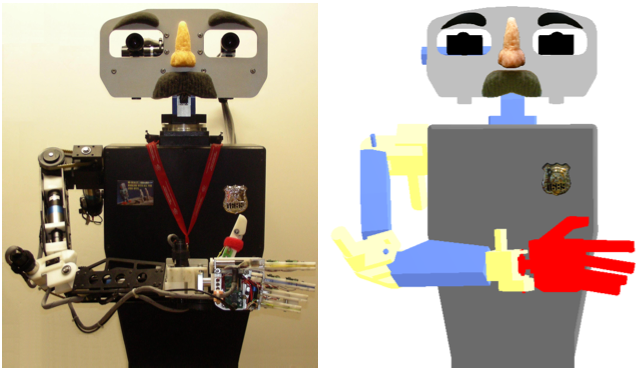
\includegraphics[scale=0.5]{figures/balta_real_cad}
\caption[Real Baltazar and its CAD model]{Real Baltazar and its CAD model (obtained with the Webots robot simulator~\cite{link:webots}).}
\label{img:balta_real_cad}
\end{figure}

\begin{figure}
\centering
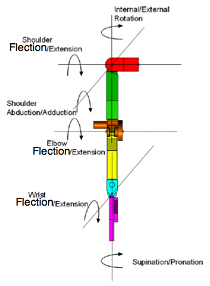
\includegraphics{figures/balta_arm_scheme} 
\caption[Scheme of Baltazar anthropomorphic arm]{Scheme of Baltazar anthropomorphic arm with available rotation \acp{DOF}.}
\label{img:balta_arm_scheme}
\end{figure}

\begin{figure}
\centering
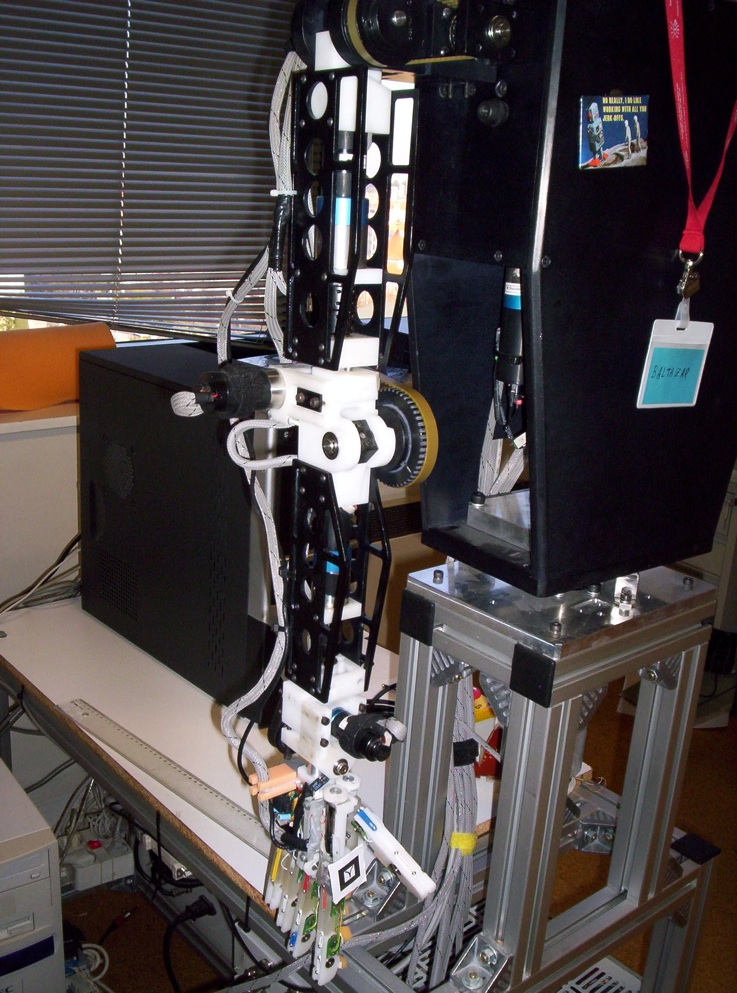
\includegraphics{figures/balta_arm_real} 
\caption[Real Baltazar anthropomorphic arm]{Real anthropomorphic arm of Baltazar.}
\label{img:balta_arm_real}
\end{figure}

Fig.~\ref{img:balta_real_cad} shows the robotic platform Baltazar in its entirety, whereas a scheme and a picture of the arm can be seen in Fig.~\ref{img:balta_arm_scheme} and in Fig.~\ref{img:balta_arm_real}, respectively.

\label{balta_ee}
The intersection between the two last motor axes, at the base of the wrist, is considered the end-effector for Baltazar.\index{Baltazar!end-effector}

Forward and inverse kinematics of the robotic arm are taken into account. This arm, which aims to replicate a human one, consists of 6 joints:
\begin{itemize}
\item 2 joints are associated with the shoulder;

\item 2 with the elbow; and

\item 2 with the wrist.
\end{itemize}

As far as this work is concerned, forward kinematics will be used as an extra tool or constraint to the iterative inverse kinematics solution which will be detailed later. The purpose is to exclude those solutions that do not respect a specific restriction imposed on the position of some joints. This is done to operate the robot easily and with no risk of damage when it is close to other objects, such as a table.

%%%%%%%%%%%%%%%%%%%%%%%%%%%%%
\subsection{Anthropomorphic Arm Forward Kinematics}
\index{Baltazar!anthropomorphic arm!forward kinematics}

\begin{table}
\caption[\acs{SDH} parameters of Baltazar anthropomorphic arm]{A possible \ac{SDH} parameterization of the anthropomorphic arm of Baltazar, derived during this thesis work in order to make use of existing robotics tools.}
\label{tab:balta_arm_sdh}
\centering
\medskip
\begin{tabular}{*{5}{l}} % table with 5 left-aligned columns
\toprule
Link $i$ & $a_i$ [cm] & $d_{i+1}$ [cm] & $\alpha_i$ [$\degree$] & $\theta_{i+1}$ [$\degree$] \\
\otoprule
$0$ & $0$ & $0$ & $\pi/2$ & $-\pi/2$ \\
\midrule
$1$ & $0$ & $0$ & $\pi/2$ & $\pi/2$ \\
\midrule
$2$ & $2.82$ & $29.13$ & $\pi/2$ & $\pi/2$ \\
\midrule
$3$ & $2.18$ & $0$ & $\pi/2$ & $\pi$ \\
\midrule
$4$ & $0$ & $26.95$ & $\pi/2$ & $\pi/2$ \\
\midrule
$5$ & $0$ & $0$ & $0$ & $-\pi/2$ \\
\bottomrule
\end{tabular}
\end{table}

A possible \ac{SDH} parameterization of Baltazar 6-\acs{DOF} arm, written down for this thesis work in a way similar to how the iCub arm kinematics was derived\footnote{\url{http://eris.liralab.it/wiki/ICubForwardKinematics}}, is shown in Table~\ref{tab:balta_arm_sdh}. Similarly, an \ac{MDH} parameterization for the anthropomorphic arm is shown in Table~\ref{tab:balta_arm_mdh}.

\begin{table}
\caption[\acs{MDH} parameters of Baltazar anthropomorphic arm]{A possible \ac{MDH} parameterization of the anthropomorphic arm of Baltazar, taken from~\cite{lopes:2004}.}
\label{tab:balta_arm_mdh}
\centering
\medskip
\begin{tabular}{*{5}{l}} % table with 5 left-aligned columns
\toprule
Joint $i$ & $a_{i-1}$ [cm] & $d_i$ [cm]& $\alpha_{i-1}$ [$\degree$] & $\theta_i$ [$\degree$] \\
\otoprule
$1$ & $0$ & $0$ & $0$ & $0$ \\
\midrule
$2$ & $0$ & $0$ & $\pi$ & $\pi/2$ \\
\midrule
$3$ & $0$ & $29.13$ & $\pi$ & $\pi/2$ \\
\midrule
$4$ & $2.82$ & $0$ & $\pi$ & $0$ \\
\midrule
$5$ & $-2.18$ & $26.95$ & $-\pi$ & $\pi/2$ \\
\midrule
$6$ & $0$ & $0$ & $\pi$ & $0$ \\
\bottomrule
\end{tabular}
\end{table}



%%%%%%%%%%%%%%%%%%%%%%%%%%%%%
\subsection{Anthropomorphic Arm Inverse Kinematics}
\index{Baltazar!anthropomorphic arm!inverse kinematics}
\label{sec:balta_arm_inv_kin}

The inverse kinematics problem is that of computing the joint angles\footnote{For a robot whose joints are all rotational, like the one used in this work.} that a robot configuration should present, given a spatial position and orientation of the end-effector. This is a useful tool for manipulator path planning, more so than forward kinematics.

One problem is that, in general, the inverse kinematic solution is non-unique, and for some manipulators no closed-form solution exists at all. If the manipulator possesses more \acp{DOF} than the number strictly necessary to execute a given task, it is called \emph{redundant} and the solution for joint angles is under-determined. On the other hand, if no solution can be determined for a particular manipulator pose, that configuration is said to be \emph{singular}. Typically, a singularity is due to an alignment of axes reducing the effective \acp{DOF}.

We address inverse kinematics in two steps. First, we set the anthropomorphic arm to the desired position (positioning of wrist); then, we change its orientation to a suitable one (orientation of hand).

Let $\mathbf{P}$ denote the desired position of the wrist, and $\mathbf{Z}$ be a null vector. In homogeneous coordinates, this means that:
%
\begin{gather}
\mathbf{P} = \begin{bmatrix} x & y & z & 1 \end{bmatrix}^T, \\
\mathbf{Z} = \begin{bmatrix} 0 & 0 & 0 & 1 \end{bmatrix}^T.
\end{gather}

The position of the wrist, $\mathbf{P}$, can be related to the various joint angles by cascading the different homogeneous coordinate transformation matrices:
%
\begin{equation}\label{eq:wrist_pos}
\mathbf{P} = \prod_{i=0}^5 \quad \leftidx{^i}{\mathbf{T}}_{i+1} \quad \mathbf{Z},
\end{equation}
%
where, as per Eq.~\ref{eq:transf}, $\leftidx{^i}{\mathbf{T}}_{i+1}$ denotes homogeneous transformation between frames $i+1$ and $i$.

In order to achieve a desired 3D location, the first four joints of the arm (counting from the shoulder) must be set to a specific position. Like~\cite{lopes:2004}, we will use the following transcendental result iteratively in order the determine these positions. Equation
%
\begin{equation}
a \cos(\theta) + b \sin(\theta) = c 
\end{equation}
%
has solutions
%
\begin{equation}\label{eq:transc}
\theta = 2 \arctan \left( \frac{b \pm \sqrt{a^2+b^2+c^2}}{a+c} \right).
\end{equation}

Eq.~\ref{eq:transc} is useful for determining the joint angles of an inverse kinematics problem. Notice that this equation has two solutions: the desired joint position can be chosen accordingly to the physical limits of a joint and/or by using additional criteria (comfort, least change).

To position the arm wrist to a given position $\mathbf{P}$ in space, we need to determine the corresponding values of joints $\theta_1, \theta_2, \theta_3, \theta_4$. Given the kinematic structure of the anthropomorphic arm of Baltazar, the distance $\rho$ from the base to the wrist (end-effector) depends only on $\theta_4$. Using Eq.~\ref{eq:wrist_pos}, the following constraint holds:
%
\begin{equation}\label{eq:theta4value}
a \cos(\theta_4)+  b \sin(\theta_4) = \rho^2 - (a_2^2 + l_2^2 + l_1^2 + a_1^2),
\end{equation}
%
where
\begin{equation}
\begin{eqsystem}
a = 2 (- a_2 a_1 + l_2 l_1) \\
b = - 2 (l_2 a_1 + a_2 l_1).
\end{eqsystem}
\end{equation}

Since Eq.~\ref{eq:theta4value} is compatible with the transcendental Eq.~\ref{eq:transc}, we can determine the value of $\theta_4$.

The solution of $\theta_2$ and a constraint on $\theta_3$ are obtained from the $z$ component (third column) of $\mathbf{P}$, obtained from Eq.~\ref{eq:wrist_pos}. In order for the parameters in Eq.~\ref{eq:transc} to permit the existence of a $\theta_2$ solution, we need $\theta_3$ to be such that:
%
\begin{gather}
a^2 + b^2 + c^2 > 0 \label{eq:theta3constraint} \\
\begin{eqsystem}
a = d_2 \cos(\theta_4) + l_2 \sin(\theta_4) - d_1 \sin(\theta_3) \\
b = - d_1 \sin(\theta_4) + l_2 \cos(\theta_4) + l_1\\
c = z.
\end{eqsystem}
\end{gather}

The algorithm that computes inverse kinematics consists in initializing $\theta_3$ in such a way that the constraint of Eq.~\ref{eq:theta3constraint} holds, subsequently allowing the computation of the remaining joint angles~\cite{carreiras:predgrab}.


All the computed angle variables are tested against the two solutions of Eq.~\ref{eq:transc}, so that we can verify if the values are coherent with the physical joint limits of the anthropomorphic arm (see Table~\ref{tab:balt_arm_joints} on p.~\pageref{tab:balt_arm_joints}).

As far as hand orientation is concerned, it is sufficient to constrain the solutions to a specific \emph{plane}, by specifying a normal vector to the plane as an input of the inverse kinematics software solver. Note that, in this way, one \ac{DOF} is still free (hand palm up or hand palm down).

%%%%%%%%%%%%%%%%%%%%%
%%%%%%%%%%%%%%%%%%%%%
\section{Hardware Devices of Baltazar}
\index{Baltazar!hardware devices}

\subsection{``Flea'' Cameras}

\begin{figure}
\centering
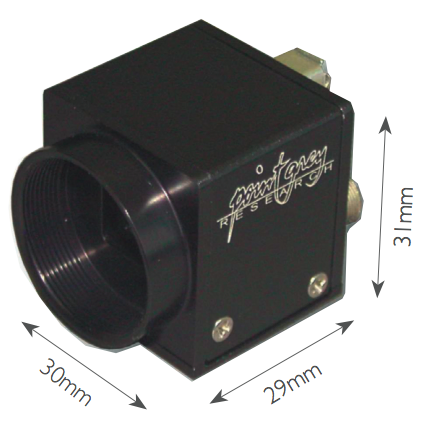
\includegraphics[scale=0.4]{figures/flea}
\caption[Point Grey ``Flea'' camera]{Point Grey ``Flea'' camera. The small dimensions of these cameras is worth noting, making it possible to employ them as (moving) humanoid eyes.}
\label{img:flea}
\end{figure}

Two colour cameras are attached on each of the eyes of Baltazar. These are ``Flea'' cameras, manufactured by Point Grey Research and displayed in Fig.~\ref{img:flea}. They are equipped with an IEEE-1394 FireWire interface and the following characteristics:
\begin{itemize}
\item very compact size: $30 \times 31 \times 29$ mm;

\item 1/3'' Sony \ac{CCD} sensor;

\item high processing speed, up to $640 \times 480$ resolution at 60 \ac{FPS};

\item external trigger, strobe output;

\item 12-bit \ac{ADC}.
\end{itemize}


\begin{figure}
\centering
\subfloat[][``Flea'' camera seen from above.]
{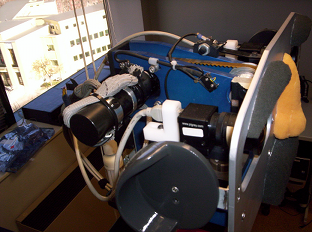
\includegraphics[width=.90\columnwidth]{figures/balta_cam_above} \label{img:balta_cam_above} } \\
%
\subfloat[][``Flea'' camera seen from below.]
{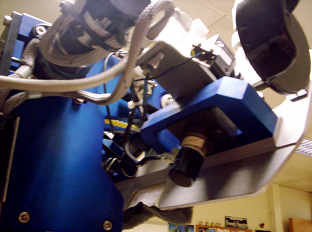
\includegraphics[width=.90\columnwidth]{figures/balta_cam_below} \label{img:balta_cam_below} }
%
\caption[Right eye Baltazar camera]{Right eye Baltazar camera as seen from two perspectives.}
\label{fig:balta_cam}
\end{figure}


%TODO: insert specification table and explain how we came to our custom params

%%%%%%%%%%%%%%%%%
\subsection{Controller Devices}

%NMCTest.exe => COM4 = hand; COM 1 = arm

\begin{figure}
\centering
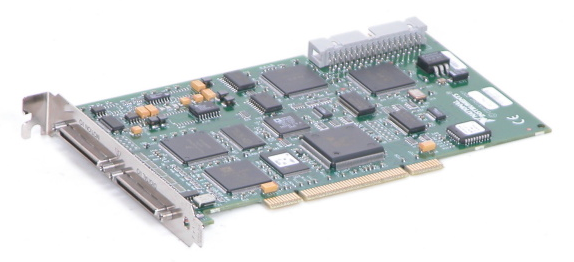
\includegraphics[scale=0.5]{figures/ni7340}
\caption[National Instruments 7340 Motion Controller]{National Instruments 7340 Stepper/Servo Motion Controller.}
\label{img:ni7340}
\end{figure}

The four \acp{DOF} of the head of Baltazar correspond to four axes or encoders; these are managed by a National Instruments PCI-7340 motion control board, shown in Fig.~\ref{img:ni7340}.

The 7340 controller is a combination servo and stepper motor controller for PXI, Compact PCI, and PCI bus computers. It includes programmable motion control for up to four independent or coordinated axes of motion, with dedicated motion I/O for limit and home switches and additional I/O for general-purpose functions. Servo axes can control:
\begin{itemize}
\item servo motors;

\item servo hydraulics;

\item servo valves and other servo devices.
\end{itemize}

Servo axes always operate in closed-loop mode. These axes use quadrature encoders or analog inputs for position and velocity feedback and provide analog command outputs with a standard range of $\pm 10$ V.

Stepper axes of the 7340 controller, on the other hand, can operate in open- or closed-loop mode. In closed-loop mode, they use quadrature encoders or analogue inputs for position and velocity feedback (in closed-loop only), and they provide step/direction or clockwise/counter-clockwise digital command outputs. All stepper axes support full, half, and microstepping applications.

The 7340 controller reflects a dual-processor architecture that uses a 32-bit CPU, combined with a \ac{DSP} and custom \acp{FPGA}, all in all providing good performance.

\bigskip

With regards to application software for this controller, the bundled tool NI-Motion is used. NI-Motion is a simple high-level programming interface (\acs{API}) to program the 7340 controller. Function sets are available for LabVIEW~\cite{link:labview} and other programs.

LabVIEW is a platform and development environment for a visual programming language (also from National Instruments) called ``G''. 

%\subsection{Limb control board}

In order to actuate the anthropomorphic arm and hand of Baltazar, another control board is mounted on the platform. The \ac{NMC} communication protocol\footnote{\url{http://www.jrkerr.com/overview.html}} is used to control the six joints of the limbs of the robot.

%\verb!TODO: add picture!

\begin{table}
\caption[Joint angles in Baltazar arm server]{Joint angles as available in Baltazar arm \acs{YARP} server. The ``physical limits'' are the actual angle limitations of the real robot joints, while the ``original bounds'' column indicates the limits that had been theoretically planned in Lopes \emph{et al.}~\cite{lopes:2004}, for the sake of historical reference.

All angles are expressed in degrees.}
\label{tab:balt_arm_joints}
\centering
\medskip
\begin{tabular}{*{5}{l}} % table with left-aligned columns
\toprule
encoder & description & arm joint & physical limits & original bounds \\
\otoprule
1 & shoulder abduction/adduction & 1 & [-45 35] & [-45 135] \\
\midrule
2 & shoulder extension/flection & 2 & [-40 5] & [-110 10] \\
\midrule
3 & not used & - & - & - \\
\midrule
4 & torso rotation & - & - & - \\
\midrule
5 & shoulder external/internal rotation & 3 & [-90 0] & [-90 0] \\
\midrule
6 & elbow extension/flection & 4 & [-90 0] & [-90 0] \\
\midrule
7 & arm pronation/supination & 5 & [-80 80] & [-90 90] \\
\midrule
8 & wrist extension/flection & 6 & [-29 45] & [-45 45] \\
\bottomrule
\end{tabular}
\end{table}

%%%%%%%%%%%%%
%%%%%%%%%%%%%
\section{Software Setup}

During the development of a piece of software, particularly if it is a project involving different people and institutions as well as operating systems and hardware, one should keep in mind certain basic principles of software engineering\index{software engineering} at all times:
\begin{itemize}
\item high cohesion;

\item low coupling

\item explicit interfacing;

\item information hiding.
\end{itemize}

Some software libraries that were largely employed in the development of this project (chiefly the \acs{YARP} set of libraries) will now be briefly presented.

%%%%%%%%%%
\subsection{YARP}
\label{sec:yarp} \index{YARP}

The iCub software (and other projects developed under the ``umbrella'' of the \ac{RobotCub} Consortium, such as this thesis) is potentially parallel and distributed. Apart from \acp{API} that speak directly to the hardware, the upper layers might require further support libraries, as is often necessary when programming robot systems immersed in various computer networks. In fact, many software solutions are already available~\cite[Table~1]{calisi:2008}. In the case of \ac{RobotCub}, these missing libraries include \emph{middleware}\index{middleware} mechanisms and were custom developed: their suite is called \ac{YARP}.

\ac{YARP} is open source\index{open source} and, as such, it is suitable for inclusion of newly developed iCub code. The rationale in this choice lays in the fact that having the source code available and, especially, well understood, can potentially simplify the software integration activity.

In order to facilitate the integration of code, clearly the simplest way would be to lay out a set of standards and to ask developers to strictly follow them. In a large research project like \ac{RobotCub}, the community should also allow for a certain freedom to developers, so that ideas can be tested quickly. These two requirements are somehow conflicting. Especially, they are conflicting when different behaviours are to be integrated into a single system and the integrator is not the first developer.

To allow developers to build upon the already developed behaviours, the researchers of \ac{RobotCub}\index{RobotCub} chose to layer the software and release-packaged behaviours in the form of \acp{API}. The idea is to produce behaviours that can be used without necessarily getting into the details of the middleware code employed. While for lower levels there is no much alternative than following a common middleware approach, higher levels and user level code can be developed by considering a less demanding scenario. In the latter case, modules are distributed with interfaces specified in an \ac{API}---possibly a C++ class hierarchy.

\begin{figure}
\centering
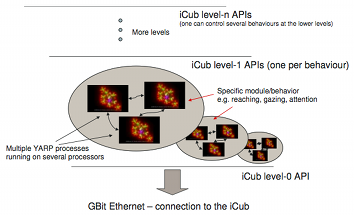
\includegraphics{figures/icub_sw_arch}
\caption[Software architecture of the iCub]{Software architecture of the iCub (and \acs{RobotCub}).}
\label{img:icub_sw_arch}
\end{figure}

Internally, each module will unleash a set of YARP processes and threads whose complexity will be hidden within the module. Various levels of configuration are possible. In one case, the given module would be capable of running on a single processor machine. This is a tricky and difficult choice since in many cases the behaviour of the robot relies explicitly on timing, synchronization, and performances of its submodules. Considering that eventually each module is a very specialized controller, issues of real-time performances have to be carefully evaluated. The modules' \acp{API} will include tests and indications on the computational timing and additional requirements in this respect, to facilitate proper configuration and use.

Fig.~\ref{img:icub_sw_arch} exemplifies the iCub software architecture. The lowest level of the software architecture consists of the level-0 \ac{API} which provides the basic control of the iCub hardware by formatting and unformatting IP packets into appropriate classes and data structures. IP packets are sent to the robot via a Gbit Ethernet connection. For software to be compliant to the iCub, the only requirement is to use this and only this \ac{API}. The \ac{API} is provided for both Linux and Windows. The iCub behaviours/modules/skills will be developed using \ac{YARP} to support parallel computation and efficient \ac{IPC}. \ac{YARP} is both open source\index{open source} and portable (i.e., OS independent), so it fits the requirements of \ac{RobotCub} in this sense. Each module can thus be composed of several processes running on several processors. 

\ac{YARP} is an open source framework for efficient robot control, supporting distributed computation and featuring a middleware infrastructure~\cite{link:yarp, metta:yarp}.

\ac{YARP} was created for a number of reasons:
\begin{itemize}
\item computer multitasking: it is useful to design a robot control system as a set of processes running on different computers, or several central processing units (CPUs) within a single system;

\item making communication between different processes easy;

\item code decoupling and modularity: it is a good practice to maintain and reuse small pieces of code and processes, each one performing a simple task. With \ac{YARP} it is easy to write location-independent modules, which can run on different machines without code changes whatsoever;

\item possibility to redistribute computational load among CPUs, as well as to recover from hardware failures.
\end{itemize}

In particular, as far as communication is concerned, \ac{YARP} follows the \emph{Observer} design pattern\index{observer design pattern|see{publish/subscribe}} (also known as \emph{publish/subscribe}\index{publish/subscribe}; see~\cite{gamma}). One or more objects (``observers'' or ``listeners'') are registered to observe an event that may be raised by the observed object (the ``subject'').

Several \emph{port} objects deliver messages to any number of observers, i.e., to their ports.

%%%%%%%%%%%%%%%%%%%%
\subsection{Other Software Libraries}

Besides \ac{YARP}, other libraries used for the implementation that are worth mentioning are \ac{GSL}\index{GSL}, its \ac{BLAS}\index{BLAS} interfaces, and OpenCV.

\bigskip

\ac{GSL} is a software library written in C for numerical calculations. Among other things, \ac{GSL} includes an implementation of the \ac{BLAS} interface.

\ac{BLAS}~\cite{link:blas} is a set of routines for linear algebra, useful to efficiently perform operations with vectors and matrices. They are divided into:
\begin{itemize}
\item Level 1 \ac{BLAS} for vector-vector operations;

\item Level 2 \ac{BLAS} for matrix-vector operations;

\item Level 3 \ac{BLAS} for matrix-matrix operations.
\end{itemize}

During the development of this thesis, \ac{GSL} and \ac{BLAS} were used to make computations between matrices fast and robust (preventing memory leaks and segmentation faults, thus improving security\index{security}).

OpenCV~\cite{link:opencv}\index{OpenCV} is a multi-purpose \ac{CV} library originally developed by Intel. Nowadays it is free for commercial and research use (under a BSD license). This library has two characteristics that it shares with \ac{RobotCub} research and that made us choose it:
\begin{itemize}
\item being cross-platform;

\item having a focus on real-time image processing. If OpenCV finds Intel's Integrated Performance Primitives (IPP) on the working system, it will use these commercial optimized routines to accelerate itself.
\end{itemize}
%!TEX encoding = UTF-8 

\chapter{Proposed Architecture}
\label{chap:proposed_architecture}

In \ac{RobotCub}\index{RobotCub} and in this thesis project too, manipulation is seen as a means to assist perception\index{perception} under uncertainty. Often, vision alone is not enough to reliably segment\index{image segmentation} distinct objects from the background. Overlapping objects or similarity in appearance to the background can confuse many visual segmentation algorithms. Rather than defining an object in terms of its appearance or shape as a predefined model, we propose a simple framework, where only the position and orientation of a tracked object are taken into consideration. This will be done by \emph{estimating the orientation as the major axis of the best-fit enclosing ellipse\index{ellipse} that surrounds the object}.

In this section we will describe the proposed visual processing (a segmentation based on colour histograms), our 3D reconstruction technique, and the applications to object manipulation tasks.

%%%%%%%%%%%%%%
%%%%%%%%%%%%%%
\section{Visual Processing}

Using \ac{CV} to control grasping tasks is natural, since it allows to recognize and to locate objects~\cite{dufournaud:1998}. In particular, stereopsis can help robots reconstruct a 3D scene and perform visual servoing.

As discussed in Section~\ref{sec:segmentation}, the problems of object tracking and image segmentation can be handled from several different perspectives. There exist elaborate methods which implement tracking, based, for example, on: contour tracking by the means of \emph{snakes}; association techniques and matrix Eigenvalues (Eigenspace matching); maintaining large sets of statistical hypotheses; computing a convolution of the image with predefined feature detector patterns. Most of these techniques, though, are computationally expensive and not suited for our framework, which must be simple enough and be able to run in real time, such as at 30 \ac{FPS}.

So, \ac{CV} algorithms that are intended to form part of a \ac{PUI}, such as our problem and all \ac{RobotCub} research in general, must be fast and efficient. They must be able to \emph{track in real time}, yet not absorb a major share of the computational resources that humanoid robots have.

The majority of the available segmentation algorithms in literature do not cover all the needs of our objective optimally, because they do not possess all of our requirements:
\begin{itemize}
\item being able to track similar objects;

\item being robust to noise;

\item working well and reasonably \emph{fast}, since the tracking algorithm is going to be run in parallel with a considerable set of computationally heavy tasks, so that the robot arm is able to intercept and grasp objects;

\item in particular, we want to run several concurrent instances of the algorithm at the same time, so performance is an important requirement.
\end{itemize}

\bigskip

A possible approach we initially thought of was to interpret motion statistically: by performing a Bayesian interpretation of the problem, the solution of motion estimation could be translated to inferring and comparing different similarity functions, generated from different motion models.

Alternatively, we could have used the \ac{EM}\index{image segmentation!clustering!EM} algorithm\footnote{A variant of $k$-Means (see Section~\ref{kmeans}).} to choose the best model. This method is frequently employed in statistical problems, and it consists of two phases, shown in~Algorithm~\ref{algo:em}.

\begin{algorithm}
\caption{\acl{EM} (\acs{EM})}
\label{algo:em}
\begin{algorithmic}[1]
\STATE (E step) Extrapolate a parameterized likelihood.
\STATE (M step) Maximize the expected likelihood found in the E step.
\end{algorithmic}
\end{algorithm}

More precisely, in the E step we associate all the points that correspond to a randomly chosen model, and in the M step we update the model parameters basing on the points that were assigned to it. The algorithm is iterated over and over, until the model parameters converge.

The solutions recalled so far in this chapter deal with a problem that is similar to the one we want to address---on the one hand, we need to establish \emph{a~priori} the set of motion models that the object can present; on the other hand we wish to choose the best possible motion model.

\bigskip

To sum up, several different approaches for segmentation are possible; though, since the development of a tracking algorithm is not the main objective of this work (it is but an initial component of it), and performance is a strong requirement, we opted for using a simple, ready-made solution from OpenCV\index{OpenCV} (Intel Open Source Computer Vision Library,~\cite{link:opencv}), which is a library of C/C++ functions and algorithms frequently used in image processing. The method that we chose was \ac{CAMSHIFT}\index{CAMSHIFT}, detailed further down. However, some custom modifications were applied by us on the OpenCV version of \ac{CAMSHIFT}. The most relevant of them are these two: 
\begin{itemize}
\item we compute the enclosing ellipse\index{ellipse} of an object by focusing the attention on the axes and centroid of such an ellipse (rather than memorizing and transmitting a whole rectangular area, we just handle, for instance, the major axis of the ellipse);

\item we add networking capabilities to the OpenCV implementation of \ac{CAMSHIFT}, by encapsulating it into the \ac{YARP} module system (see Section~\ref{sec:yarp}) and using a middleware\index{middleware} mechanism. This makes it possible to run several instances of the tracker in parallel, for example two trackers to track an object with stereopsis\index{stereopsis}, or multiple objects.
\end{itemize}

%%%%%%%%%%%%%%%
\section{\acs{CAMSHIFT} Module}
\label{sec:camshift_module}

The \acl{CAMSHIFT} algorithm\index{CAMSHIFT}, or \acs{CAMSHIFT} for short, is based on Mean~Shift~\cite{comaniciu:1997}, which in turn is a robust, non-parametric iterative technique for finding the mode of probability distributions. Interestingly, the Mean Shift algorithm was not originally intended to be used for tracking, but it proved effective in this role nonetheless (see~\cite{bradski:1998}).

\ac{CAMSHIFT} is fast and simple; as such, it fulfils the requirements of our project. It is a technique based on colour, however, contrary to similar algorithms, \ac{CAMSHIFT} does \emph{not} take into account colour correlation, blob growing, region growing, contour considerations, Kalman filter smoothing and prediction (all of which are characteristics that would place a heavy burden on computational complexity and speed of execution).

The complexity of most colour-based tracking algorithms (other than \ac{CAMSHIFT}) derives from their attempt to deal with \emph{irregular object motion}, which can be due to:
\begin{itemize}
\item perspective\index{perception} (near objects to the camera seem to move faster than distal ones);

\item image noise;

\item distractors, such as other shapes present in the video scene;

\item occlusion\index{occlusion} by hands or other objects;

\item lighting variation.
\end{itemize}

Indeed, all of the above are serious problems that are worth studying and being modelled for certain practical applications, however the main trait of \ac{CAMSHIFT} is that it is a fast, computationally-efficient algorithms that mitigates those issues ``for free'', i.e., during the course of its own execution.

\bigskip

\begin{algorithm}
\caption{Mean Shift}
\label{algo:meanshift} \index{Mean Shift}
\begin{algorithmic}[1]
\STATE Choose a search window size.
\STATE Choose the initial location of the search window.
\STATE Compute the mean location in the search window.
\STATE Centre the search window at the mean location computed in step 3.
\STATE Repeat steps 3 and 4 until convergence (or until the mean location moves less than a preset threshold).
\end{algorithmic}
\end{algorithm}

At the beginning of this section, we mentioned that in general Mean Shift~(see Algorithm~\ref{algo:meanshift}) operates on probability distributions. Therefore, in order to track coloured objects in a video frame sequence, the colour image data has to be represented as a probability distribution~\cite{comaniciu:1997} --- to do this, \emph{colour histograms} are used.

Colour distributions that are derived from video image sequences may change over time, so the Mean Shift algorithm must be modified to dynamically adapt to the probability distribution that it is tracking at a given moment. It is here that the new, modified algorithm --\ac{CAMSHIFT}-- bridges the gap (also see~\ref{img:colour_obj_tracking}).

\bigskip

Given a colour image and a colour histogram, the image produced from the original colour image by using the histogram as a lookup table is called \emph{back-projection image}. If the histogram is a model density distribution, then the back-projection image is a probability distribution of the model in the colour image. \acs{CAMSHIFT}\index{CAMSHIFT} detects the mode in the probability distribution image by applying Mean Shift while dynamically adjusting the parameters of the target distribution. In a single image, the process is iterated until convergence---or until an upper bound on the number of iterations is reached.

A detection algorithm can be applied to successive frames of a video sequence to track a single target. The search area can be restricted around the last known position of the target, resulting in possibly large computational savings. This type of scheme introduces a feedback loop, in which the result of the detection is used as input to the next detection process. The version of \ac{CAMSHIFT} applying these concepts to tracking of a single target in a video stream is called Coupled \ac{CAMSHIFT}\index{CAMSHIFT!Coupled CAMSHIFT}.

The Coupled \ac{CAMSHIFT} algorithm as described in~\cite{bradski:1998} is demonstrated in a real-time head tracking application, which is part of the Intel OpenCV library~\cite{link:opencv}\index{OpenCV}. 

\begin{figure}
\centering
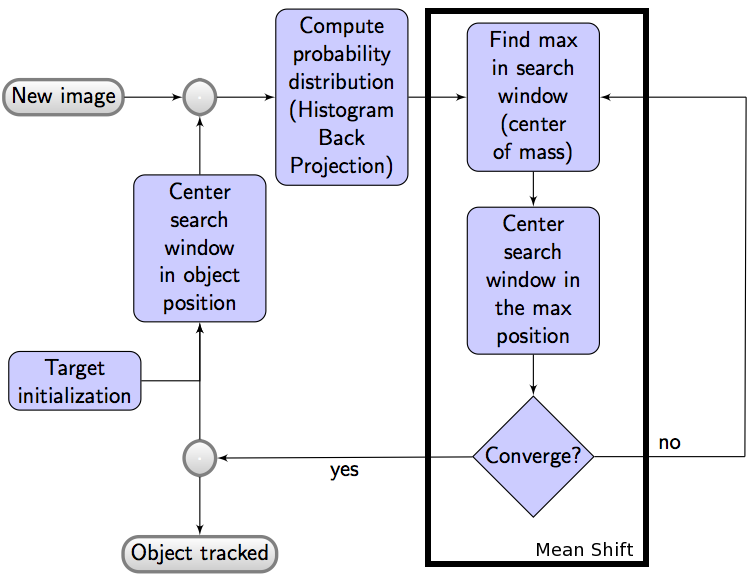
\includegraphics[scale=0.4]{figures/camshift_diag2}
\caption[Block diagram of \acs{CAMSHIFT}]{Block diagram of \ac{CAMSHIFT}.}
\label{img:camshift_diag2}
\end{figure}

% we added computation of major axis of ellipse
% use the 2 extremities as an input for other modules

%%%%%%%%%%%%%%%%%%%%%%%%%%%%%%%%%
\subsection{\acs{CAMSHIFT} and \acs{HSV} Conversion}
\index{HSV}

In order to use a histogram-based method to track coloured objects in a video scene, a probability distribution image of the desired colour present in the video sequence must first be created. For this, one first creates a model of the desired \emph{hue} by using a colour histogram.

The reason why \ac{HSV} space is better suited for our proposed perceptual interface is the following. Other colour models like \ac{RGB}, \ac{CMY}, and YIQ are hardware-oriented~\cite[p.~590]{foley}. By contrast, Smith's \ac{HSV}~\cite{smith:1978} is user-oriented, being based on the intuitive, ``artistic'' approach of tint, shade and tone.

In general, the coordinate system of \ac{HSV} is cylindrical; however, the subset of space within which the model is defined is a hexcone\footnote{Six-sided pyramid.}, as in Fig.~\ref{fig:hsv}. The hexcone model is intended to capture the common notions of hue, saturation and value:
\begin{itemize}
\item Hue is the hexcone dimension with points on it normally called red, yellow, blue-green, etc.;

\item Saturation measures the departure of a hue from achromatic, i.e., from white or gray;

\item Value measures the departure of a hue from black (the colour or zero energy).
\end{itemize}
These three terms are meant to represent the artistic ideas of hue: tint, shade and tone.

The top of the hexcone in Fig.~\ref{fig:hsv} corresponds to $V = 1$, which contains the relatively bright colours. Descending the V axis gives smaller hexcones, that correspond to smaller (darker) \ac{RGB} subcubes in Fig.~\ref{fig:rgb}.

%The colours of the $V = 1$ plane are not all of the same perceived brightness, however: colour plates II.7 and II.8 show the colour model.

\begin{figure}
\centering
\subfloat[][RGB colour cube.]
{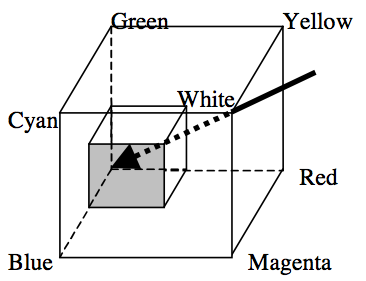
\includegraphics[width=.45\columnwidth]{figures/rgb} \label{fig:rgb} } \quad
% %necessary to prevent line break
\subfloat[][HSV colour system.]
{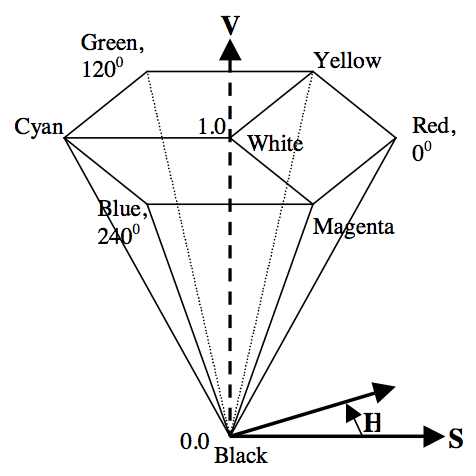
\includegraphics[width=.45\columnwidth]{figures/hsv} \label{fig:hsv} }

\caption[RGB and HSV colour spaces]{RGB and HSV colour spaces. In the single-hexcone HSV model, the $V = 1$ plane contains the RGB model's $R = 1, G = 1$, and $B = 1$ planes in the regions shown.}
\label{fig:rgb-hsv}
\end{figure}

The \ac{HSV} colour space is particularly apt to capture senses and perception, more so than \ac{RGB}. \ac{HSV} corresponds to projecting standard Red, Green, Blue colour space along its principle diagonal from white to black \cite{smith:1978}, as seen looking at the arrow in Fig.~\ref{fig:rgb}. As a result, we obtain the hexcone in Fig.~\ref{fig:hsv}. 
\ac{HSV} space separates out Hue (colour) from Saturation (i.e., how concentrated the colour is) and from brightness. In the case of \ac{CAMSHIFT}, we create our colour models by taking 1D histograms (with 16 bins) from the H channel in \ac{HSV} space.


% check:
% ignore (?) Hue component => invariant to colour
% ignore (?) Intensity component => invariant to illumination

\ac{CAMSHIFT}\index{CAMSHIFT} is designed for dynamically-changing distributions. These occur when objects in video sequences are being tracked and the object moves so that the size and location of the probability distribution changes in time. The \ac{CAMSHIFT} algorithm adjusts the search window size in the course of its operation. Instead of a set or externally adapted window size, \ac{CAMSHIFT} relies on the zeroth moment information, extracted as part of the internal workings of the algorithm, to \emph{continuously} adapt its window size within or over each video frame.

The zeroth moment can be thought of as the distribution ``area'' found under the search window~\cite{bradski:1998}. Thus, window radius, or height and width, is set to a function of the zeroth moment found during search. \ac{CAMSHIFT}, outlined in Algorithm~\ref{algo:camshift}, is then calculated using any initial non-zero window size. 

\begin{algorithm}
\caption{\acs{CAMSHIFT}}
\label{algo:camshift}
\begin{algorithmic}[1]
\STATE Choose the initial location of the search window.
\STATE Perform Mean Shift as in Algorithm~\ref{algo:meanshift}, one or more times. Store the zeroth moment.
\STATE Set the search window size equal to a function of the zeroth moment found in Step~2.
\STATE Repeat Steps~2 and~3 until convergence (mean location moves less than a preset threshold). 
\end{algorithmic}
\end{algorithm}


%%%%%%%%%%%%%%%%%%%%%%%%%%
%%%%%%%%%%%%%%%%%%%%%%%%%%
\section{3D Reconstruction Approach}
\label{sec:3d_recon_approach}\index{3D reconstruction}

In order for a humanoid robot to be able to do things in the world, it requires to have a tridimensional perception, which is what we want to accomplish in this module, in a precise yet simple and efficient (fast) way.

The anthropomorphic head of Baltazar (Fig.~\ref{img:balta_head_real}, p.~\pageref{img:balta_head_real}) has two cameras, mounted in a way similar to the eyes of a human being (Fig.~\ref{fig:balta_cam}, p.~\pageref{fig:balta_cam}).

The notion of \emph{depth} is thus obtained from the combination of information that comes from the two cameras. In this section, we will explain a method to determine the coordinates of one point in the area that is visible from both cameras at a given moment. In particular, we want to reconstruct the 3D coordinates of two points for each object, corresponding to the two extremities of the major axis of the best-fit ellipse to the object. This visual simplification facilitates real-time performances and at the same time it opens the way for manipulation tasks.

%\bigskip

%%%%%%%%%%%%%%%%%%%%%%%%%%%%%%%%
\subsection{From Frame Coordinates to Image Coordinates}

A digitalized image is usually stored in a framebuffer which can be seen as a matrix of pixels with $W$ columns (from ``width'') and $H$ rows (from ``height'').

\begin{figure}
\centering
\includegraphics[scale=0.55]{figures/image_coords}
\caption[Image coordinates]{Image coordinates.}
\label{img:image_coords}
\end{figure}

Let $(i,j)$ be the discrete frame coordinates of the image with origin in the upper-left corner, $(O_x,O_y)$ be the focal point of the lens (the intersection between the optical axes and the image plane) in the frame coordinates, and $(x,y)$ be the image coordinates, as illustrated in Fig~\ref{img:image_coords}.

Image coordinates relate to frame coordinates in this way:
\begin{gather}
x = (i - O_x) \cdot S_x \\
y = (j - O_y) \cdot S_y
\end{gather}
where $S_x,S_y$ are the horizontal and vertical distances of two adjacent pixels in the framebuffer.

\bigskip


An \emph{a priori} hypothesis is that we know the relative displacement of the two cameras (rotation and translation) at all times. This makes sense, as we can continuously update the angle values in our software module, receiving instantaneous values from the robot encoders, for example at a frequency of one update per second.

The matrix of intrinsic parameters\index{intrinsic parameters} of a camera, which sets the relationship between a 3D point and the pixels in a sensor, will not be explicitly computed in this project. In other words, we avoid the calibration\index{calibration} phase. The only aspects that we will consider are:
\begin{itemize}
\item image resolution;

\item focal distance\index{focal distance}; and

\item pixel size.
\end{itemize}




% passage from reconstruction to triangulation?
% triangulation:

In stereo analysis\index{stereopsis}, \emph{triangulation}\index{triangulation} is the task of computing the 3D position of points in the images, given the disparity map and the geometry of the stereo setting. The 3D position $(X, Y, Z)$ of a point $\mathbf{P}$ can be reconstructed from the perspective projection\index{perspective projection} (see Fig.~\ref{img:perspective_geom}, p.~\pageref{img:perspective_geom}) of $\mathbf{P}$ on the image planes of the cameras, once the relative position and orientation of the two cameras are known.

For example, if we choose the 3D world reference frame to be the left camera reference system, then the right camera is translated and rotated with respect to the left one, therefore six parameters will describe this transformation.

In the most general case, the right camera can be rotated with respect to the left one (or vice versa) in three directions.


\bigskip

% triangulation.webarchive started here
%%%%%%%%%%%%%%%
%\subsection{Camera Model}

For 3D reconstruction\index{3D reconstruction}, we use a pinhole camera model\index{pinhole camera model} like the one in Fig.~\ref{img:pinhole}.

\begin{figure}
\centering
\includegraphics[scale=0.55]{figures/pinhole}
\caption[Pinhole camera model]{Pinhole camera model.}
\label{img:pinhole}
\end{figure}

The relationships that exist between the world coordinates of a point $\mathbf{P} = (X, Y, Z)$ and the coordinates on the image plane $(x, y)$ in a pinhole camera are
%
\begin{gather}
x = F \cdot X / Z \\
y = F \cdot Y / Z
\end{gather}
%
where lower-case letters refer to \emph{image} position, upper-case ones to \emph{world} position (in metres), and $F$ is the focal distance\index{focal distance} of the lens (also in metres).


Considering the two cameras and referring as $B$ to the baseline (distance between the optical centres of them), we can now obtain the missing coordinate $Z$:
%
\begin{gather}
y_L = \frac{F Y_L}{Z_L} \\
Y_R = Y_L - B \\
Z_L = Z_R = Z \\
y_R = \frac{F Y_R}{Z_R} = F \frac{Y_L - B}{Z} \\
y_L - y_R = F \frac{B}{Z} \Longleftrightarrow Z = \frac{F B}{y_L - y_R}.
\end{gather}


We will now analyze the case in which the two cameras are in an arbitrary relative orientation. A description of various vergence\index{vergence} situations can be consulted in~\cite{bernardino:1999}.

\begin{figure}
\centering
\includegraphics{figures/vergence}
\caption[3D reconstruction scheme]{3D reconstruction scheme for a stereo pair of cameras with arbitrary vergence.}
\label{img:vergence}
\end{figure}

Looking at Fig.~\ref{img:vergence}, we can thus write down the following equations for the $Z$ coordinate:
%
\begin{gather}
\tan (\theta_L + x_L / F) = \frac{B/2}{Z} \\
\tan (\theta_R + x_R / F) = \frac{B/2}{Z} \\
Z = \frac{B}{\tan(x_L / F + \theta_L) - \tan(x_R / F + \theta_R)}.
\end{gather}

As for the $X$ coordinate, we obtain:
%
\begin{gather}
\tan(\theta_L + x_L / F) = \frac{X_L}{Z} \\
\tan(\theta_R + x_R / F) = \frac{X_R}{Z} \\
X = - \frac{Z}{2} \bigl[ \tan(x_L / F + \theta_L) + \tan(x_R / F + \theta_R) \bigr].
\end{gather}

Finally, the 3D reconstructed coordinate $Y$ is obtained like this:
%
\begin{gather}
Z_{R}' = Z / \cos \theta_R \\
Z_{L}' = Z / \cos \theta_L \\
Y = \frac{Z y_R}{2 F \cos \theta_R} + \frac{Z y_L}{2 F \cos \theta_L}
\end{gather}










In order to determine the coordinates of an object in a fixed reference frame, it is necessary to consider the forward kinematics of the head\index{Baltazar!head} of Baltazar (see Section~\ref{sec:balta_head}). From coordinates that are expressed in the image plane, we want to obtain coordinates in a fixed reference frame (a frame attached to the robot torso, which does not move).

Recall the scheme of Baltazar head, illustrated in Fig.~\ref{img:balta_head_scheme}. The expression given in Eq.~\ref{eq:im2fix} was obtained from geometrical analysis, and it provides a relationship between coordinates in the image plane (of one of the two cameras) with the coordinates expressed in a fixed frame.

\begin{equation}\label{eq:im2fix}
{\mathbf{P}}_l = {\mathbf{R}}_l (\mathbf{P} - {\mathbf{t}}_l).
\end{equation}

For the sake of simplicity, Eq.~\ref{eq:im2fix} refers to the left camera case, thus the $l$ subscript. The rotation and translation matrices are, in particular, equal to
%
\begin{equation}
\begin{split}
{\mathbf{R}}_l =	&\begin{bmatrix}
				c_p c_l - c_t s_p s_l	&	- s_p s_t	&	c_t c_l s_p + c_p s_l \\
				- s_t s_l			&	c_t		&	c_l s_t \\
				- c_l s_p - c_p c_t s_l&	- c_p s_t	&	c_p c_t c_l - s_p s_l
				\end{bmatrix}; \\
{\mathbf{t}}_l =		&\begin{bmatrix}
				- B' c_l - t_Y s_t s_l + t_Z (- c_l s_p - c_p c_t s_l) \\
				t_Y c_t - t_Z c_p s_t \\
				t_Y c_l s_t - B' s_l + t_Z (c_p c_t c_l - s_p s_l)
				\end{bmatrix}
\end{split}
\end{equation}
%
where $B' = B/2$ (half the baseline distance).






%%%%%%%%%%%%%%%%%%%
%\subsection{Image Projection Model}
%\subsection{Transformation into World Coordinates}

\index{3D reconstruction}
From a geometrical point of view, the camera sensors mounted on the Baltazar head simply measure \emph{relative positions}; these two cameras are used to calculate the position of objects within their workspace, relative to their optical centre. Thus, a 3D point is mapped onto a two-dimensional space, by the means of its projection on the image plane. It is precisely in this way that we obtain the 2D coordinates of a pair of stereo cameras: the resulting coordinates derive from a 3D point located in the surrounding of Baltazar.






%TODO:
% http://eris.liralab.it/wiki/ICubFowardKinematics_right
%- how Baltazar's head calibration works
%- how we compute world-to-camera(s) matrices
%- perspective (not orthographic) projection
%- optical rays
%- software analysis and design; brief UML (classes)
%- software -> Vectors, ports closing gracefully
%- why multiprocess instead of multithread
%- complexity: where is the bottleneck?
%- drawback: can't track rotationally-symmetric objects
%- how we computed new camera parameters for Dragonfly camera with custom res

%%%%%%%%%%%%%%%%%
\subsection{3D Pose Estimation}
\index{3D reconstruction}

Consider now a \emph{target object} placed in front of the robot; tracking is accomplished by running two \ac{CAMSHIFT}\index{CAMSHIFT} processes. Let points $\{p_1, p_2\}_l^{\mathrm{target}}$ and $\{p_1, p_2\}_r^{\mathrm{target}}$ be the extremities of the major ellipse axis expressed in the 2D coordinate frame of the left and right tracker, respectively\footnote{The same considerations apply for stereo tracking and 3D reconstruction of the robot \emph{hand}, but for the sake of simplicity only the target object case is explained here. From now on, the ``target'' exponent in the notation is therefore omitted.}.

A 3D reconstruction process receives the coordinates of the four points $\{p_1, p_2 \}_{l,r}$ as inputs, along with the instantaneous head joint angle values of the robot, used to compute the time-varying extrinsic camera parameter matrices: not just the target object, but also the robot cameras may be moving during experiments. Transformation matrices $\leftidx{^w}{\mathbf{T}}_l$ and $ \leftidx{^w}{\mathbf{T}}_r$ represent the roto-translations occurring, respectively, from the left and right camera reference frame to the world (torso) reference frame, as shown in Fig.~\ref{img:balta_head_transf}.

\begin{figure}
\centering
\includegraphics{figures/recon_module}
\caption[3D reconstruction software module scheme]{3D reconstruction software module scheme, outlining the data that are passed as inputs/outpus among \ac{YARP} modules.}
\label{img:recon_module}
\end{figure}

Fig.~\ref{img:recon_module} shows how the 3D reconstruction\index{3D reconstruction} module works. It receives inputs from two \ac{CAMSHIFT}\index{CAMSHIFT} trackers (one per each eye), it receives the instantaneous head joint angles (with which it builds transformation matrices), then finally it computes estimated coordinates and orientation of a tracked object.

Thanks to how \ac{YARP}\index{YARP} is designed, we can easily run various concurrent instances of this modules in parallel. Specifically, in the grasping preparation (visual servoing) phase we will be interested in 3D reconstructing the target object and the robot hand at the same time.

Once the reconstruction is computed, 3D coordinates of $\{ p_1, p_2\}$ are obtained.
The difference vector $p_1 - p_2$ encodes the orientation of the target.


\begin{figure}
\centering
\includegraphics[scale=0.5]{figures/balta_head_transf}
\caption[Structure of Baltazar head with transformation matrices]{Mechanical structure of Baltazar head, its reference frames and points of interest. Transformation matrices are highlighted in green.}
\label{img:balta_head_transf}
\end{figure}












%%%%%%%%%%%%%%%%%%%%%%
\section{Object Manipulation Approaches}
\index{manipulation}

% how we implement concurrency, how we avoid deadlocks and problems
% reaching FSM

% why our algorithms are good


%TODO:
%- object orientation => hand orientation
%- MATLAB simulation of arm to study fw.kin., with studied SDH params

As mentioned in p.~\pageref{intro:reaching_phases}, in this work we consider two distinct phases for a manipulation task:

\begin{description}
\item[reaching preparation:]\index{reaching} this phase aims at bringing the robot hand to the vicinity of the target. It is applied whenever a target is identified in the workplace but the hand is not visible in the cameras. The measured 3D target position is used, in conjunction with the robot arm kinematics, to place the hand close to the target. Inevitably, there are mechanical calibration errors between arm kinematics and camera reference frames, so the actual placement of the hand will be different from the desired one. Therefore, the approach is to command the robot not to the exact position of the target but to a distance safe enough to avoid undesired contact both with the target and the workspace.

\item[grasping preparation:]\index{grasping} in this phase, both target and hand are visible in the camera system and their posture can be obtained by the methods previously described. The goal is now to measure the position and angular error between target and hand, and use a \ac{PBVS} approach to make the hand converge to the target. The features used in such an approach are 3D parameters estimated from image measurements---as opposed to \ac{IBVS}\index{Visual Servoing!Image-Based Visual Servoing}, in which the features are 2D and immediately computed from image data.
\end{description}

Reaching preparation is relatively easy, since in this phase we just position the arm to the vicinity of the target object (within a threshold of 20 cm). The arm starts moving from a predefined position outside of the field of view of the two cameras, and it reaches the position estimated by the inverse kinematics solver.

On the other hand, there are two peculiarities in the presented grasping preparation approach:
%
\begin{itemize}
\item Normally, \ac{PBVS}\index{Visual Servoing!Position-Based Visual Servoing} requires the 3D model of the observed object to be known~\cite{hutchinson:1996}, but in our framework one gets rid of this constraint: by using the stereo reconstruction technique explained above, the only condition to prepare the servoing task is that the \ac{CAMSHIFT} trackers are actually following the desired objects---whose models are \emph{not} known beforehand.

\item Classical \ac{PBVS} applications consider that target and end-effector positions are measured by different means, e.g. target is measured by the camera and end-effector is measured by robot kinematics. This usually leads to problems due to miscalibrations between the two sensory systems. Instead, in this work, target and hand positions are measured by the camera system in the same reference frame, therefore the system is robust to calibration errors.
\end{itemize}

\begin{figure}
\centering
\includegraphics{figures/cross_prod2}
\caption[Cross product between hand and target orientations]{Unit vector of the target object along its orientation axis (purple); unit vector and orientation of robot hand (red); third axis resulting from their cross product, and corresponding unit vector (green).}
\label{img:cross_prod2}
\end{figure}

Having computed 3D position and orientation of both a target object and of the robot hand, features suitable for the application of the \ac{PBVS}\index{Visual Servoing!Position-Based Visual Servoing} technique must be obtained. As described in~\cite{chaumette:visual1}, the robot arm can be controlled by the following law\index{control law}:
%
\begin{equation}\label{eq:cross_prod}
\begin{cases}
\mathbf{v} = -\lambda \left( \left( \mathbf{t}_\textrm{target} - \mathbf{t}_\textrm{hand} \right) + \left[ \mathbf{t}_\textrm{hand}\right]_{\times} \vartheta \mathbf{u} \right)\\
\mathbf{\omega} = -\lambda  \vartheta \mathbf{u}
\end{cases}
\end{equation}
%
where $\mathbf{v}$ and $\mathbf{\omega}$ are the arm linear and angular velocities, $\lambda$ establishes the trajectory convergence time,  $\mathbf{t}_\textrm{target}$ and $\mathbf{t}_\textrm{hand}$ are the target and hand positions, $\left[ \cdot \right]_{\times}$ is the associated skew-symmetric matrix of a vector; $\vartheta, \mathbf{u}$ are the angle-axis representation of the rotation required to align both orientations. Other control laws can be applied to this problem, but they normally rely on an angle--axis parameterization of the rotation.\index{angle--axis parameterization}

It is possible to calculate the required angle $\vartheta$ and axis $\mathbf{u}$ by applying a simple \emph{cross product rule} between the normalized hand and target orientation vectors:
%
\begin{equation}
%\mathbf{u} = o_{\textrm{target}} \times o_{\textrm{hand}} \qquad\textrm{and}\qquad \vartheta = \arcsin \| \mathbf{u} \|_{2}
\begin{cases}
\mathbf{u} = {\mathbf{o}}_{\textrm{target}} \times {\mathbf{o}}_{\textrm{hand}}\\
\vartheta = \arcsin \| \mathbf{u} \|_{2}
\end{cases}
\label{eq:theta_angle}
\end{equation}
%
where $\| \cdot \|_{2}$ is the Euclidean norm, ${\mathbf{o}}_{\textrm{target}}$ is a unit vector in the direction of the target object's reconstructed\index{3D reconstruction} orientation and ${\mathbf{o}}_{\textrm{hand}}$ is a unit vector in the direction of the hand's reconstructed orientation (see Fig.~\ref{img:cross_prod2}).
%!TEX encoding = UTF-8 

\chapter{Experimental Results}
\label{chap:experimental_results}

This chapter contains experimental results obtained by testing the programs that were written for this thesis. The whole project was carried out at Computer and Robot Vision Laboratory~\cite{link:vislab}, Institute for Systems and Robotics, Instituto Superior T\'{e}cnico, Lisbon (Portugal) for eight months during 2008.

All the tests were performed on the machine that is attached to the Baltazar\index{Baltazar} robotic platform: a personal computer with a Dual Intel Xeon 3.20GHz processor, 1GB of RAM, running Microsoft Windows XP Pro SP2.

The development environment adopted was Microsoft Visual Studio 2005, also providing a graphical debugging interface for C++.

%%%%%%%%%%%%%%%%%%%
%%%%%%%%%%%%%%%%%%%
\section{Segmentation and Tracking}

\begin{figure}[h]
\centering
\includegraphics{figures/0619grey}
\caption[\acs{CAMSHIFT} tracking experiment]{\ac{CAMSHIFT} tracking experiment, with a grey sponge.}
\label{img:0619grey}
\end{figure}

Fig.~\ref{img:0619grey} shows an early version of the custom modified \ac{CAMSHIFT}\index{CAMSHIFT} tracker while running during a video experiment. The best-fit enclosing ellipse is drawn in red, the major axis in blue.

The major axis of the ellipse\index{ellipse} represents an estimation of the target object orientation. One can see that such axis is not completely parallel to the long edges of the cuboid sponge: this is due to previous motion and frames that cause an oscillatory nature of the ellipse (axes).

Furthermore, we can see the estimated extremities of the major axis ($p_1$ and $p_2$) marked with green circles. Note that this type of experiments did not yet take into account the manipulation (reaching and grasping) of objects, thus the object centroid is neither estimated nor visually marked.

All in all, this first experiment (which involved only one instance of \ac{CAMSHIFT}\index{CAMSHIFT} tracker running at a time---no stereo vision yet) proved quite successful. The tracked object, a grey sponge, was tracked continuously for several minutes. When the object was shaken (rotated) very fast in the experimenter's hand, it was still tracked. This means that each iteration of \ac{CAMSHIFT} managed to use the colour histogram successfully for its search. On the other hand, there were some stability issues with the major ellipse of the axis or when the object was occluded for a few seconds (the tracker would not completely lose it, but its tracked region would shrink to the very small visible portion of the sponge during the occluded sequence, predictably making the axis shake between various orientations).



\begin{figure}
\centering
\subfloat[][Second \ac{CAMSHIFT} tracking experiment screenshot.]
{\includegraphics[width=.40\columnwidth]{figures/1225camshift_green} \label{img:1225camshift_green} } \quad
% %necessary to prevent line break
\subfloat[][16-bin \ac{CAMSHIFT} colour histogram used for iterative searches during all of the experiment of Fig~\ref{img:1225camshift_green}.]
{\includegraphics[width=.50\columnwidth]{figures/1225histo} \label{img:1225histo} }
%
\caption[Second \acs{CAMSHIFT} tracking experiment]{Another \ac{CAMSHIFT} tracking experiment, with a green sponge.}
\label{img:1225camshift_exp}
\end{figure}

Fig.~\ref{img:1225camshift_exp} shows the execution of another \ac{CAMSHIFT} tracking task. Here, we are computing (and displaying) not the reconstructed extremities $p_1$ and $p_2$ of the major axis of the ellipse\index{ellipse}, but rather $p_1$ and the estimated object centroid. Fig.~\ref{img:1225histo} shows the 16-bin colour histogram after it has been initialized for this experiment (green is the colour the tracker will look for, at every iteration). Note that the histogram remains constant during the whole experiment, also providing some robustness against occlusions\index{occlusion}.


%%%%%%%%%%%%%%
%%%%%%%%%%%%%%
\section{3D Reconstruction}
\index{3D reconstruction}\index{stereopsis}

\begin{figure}[h]
\centering
\includegraphics[scale=0.4]{figures/0509recon}
\caption[3D reconstruction experiment]{3D reconstruction experiment.}
\label{img:0509recon}
\end{figure}

In Fig.~\ref{img:0509recon} we can see the output of the 3D reconstruction module during an experiment. Three windows are visible:
\begin{itemize}
\item left eye \ac{CAMSHIFT} tracker;

\item right eye \ac{CAMSHIFT} tracker; and

\item 3D reconstruction module output.
\end{itemize}

As far as the two trackers are concerned, we can see an optimal behaviour and drawing of the ellipses with their respective major axes. This contrasts with previous tracking experiments such as Fig.~\ref{img:0619grey} for a number of reasons: first of all, the tracked sponge is not moving now. Because we were interested in measuring and judging the quality of our 3D reconstruction\index{3D reconstruction}, in this experiment we chose a static scenario (there was some minor flickering and oscillation in the camera views during the video, but it was a negligible phenomenon, as the tracked axis kept stable throughout the whole experiment). Secondly, the tracked object was completely in front of the white table that is in front of Baltazar\index{Baltazar}---greatly facilitating colour segmentation\index{image segmentation}.

The most important part of this experiment, though, is the behaviour of the 3D reconstruction\index{3D reconstruction} module. It is the black window with white text at the bottom of Fig.~\ref{img:0509recon}. The first three lines of text, written in capital letters, contain numerical values used internally by the 3D reconstruction module: coordinates in pixels, angles in degrees and lengths in metres. Then, the coordinates of the two extremities of the reconstructed axis ($p_1$ and $p_2$) are printed, in a $(X, Y, Z)$ world reference frame, where $Z$ is positive in the direction in front of the face of Baltazar. This means, for example, that a coordinate of
\[
Z = 0.280
\]
(metres) corresponds to 28 cm in front of the robot torso, on the white table.

The 3D reconstructed coordinates are correct in this experiment: they were checked with a ruler and the error along all the three dimensions was small (less than 5 cm).

Finally, the orientation of the target object (encoded as the different between reconstructed $p_1$ and reconstructed $p_2$) is printed.



% Paulo's:
%\begin{figure}
%\centering
%\subfloat[][$x$ error.]
%{\includegraphics[width=.70\columnwidth]{figures/recon_error_x} \label{fig:recon_error_x} } \\
%\subfloat[][$y$ error.]
%{\includegraphics[width=.70\columnwidth]{figures/recon_error_y} \label{fig:recon_error_y} } \\
%\subfloat[][$z$ error.]
%{\includegraphics[width=.70\columnwidth]{figures/recon_error_z} \label{fig:recon_error_z} }
%
%\caption[3D reconstruction error during tracking]{3D reconstruction error while tracking a moving object.}
%\label{fig:recon_error}
%\end{figure}





%%%%%%%%%%%%%%%%%%%
%%%%%%%%%%%%%%%%%%%
\section{Object Manipulation Tasks}
\index{manipulation}

%%%%%%%%%%%%%%%%%%
\subsection{Reaching Preparation}
\index{reaching}

\begin{figure}[h]
\centering
\includegraphics[scale=0.5]{figures/10xxcininv}
\caption[Object manipulation: inverse kinematics experiment]{Object manipulation: inverse kinematics solver experiment.}
\label{img:10xxcininv}
\end{figure}

Recall (p.~\pageref{intro:reaching_phases}) that in accordance to our perceptual framework we have split the reaching task in two distinct phases:
\begin{description}
\item[reaching preparation:] an open-loop ballistic phase to bring the manipulator to the vicinity of the target, whenever the robot hand is not visible in the robot's cameras;

\item[grasping preparation:] a closed-loop visually controlled phase to accomplish the final alignment to the grasping position.
\end{description}

We shall now focus on the first problem, reaching preparation. In this phase our aim is to position the anthropomorphic arm of Baltazar, initially outside of the cameras' field of view, in the ``vicinity'' of the target. To start off, we define this vicinity as the 3D reconstructed coordinates of the centroid of the target object, minus a safety threshold of 20 cm along the horizontal axis (parallel to the table and to the ground, directed towards the right of the robot, from its own point of view). So, for this phase to be successful, we need to position the robot wrist at 20 cm from the object centroid. A necessary condition to accomplish this, is to solve the robot arm inverse kinematics for the desired hand position coordinates.

Fig~\ref{img:10xxcininv} shows a number of inverse kinematics solutions found for Cartesian coordinates
\[
X = 23, Y = -42, Z = 22 \quad \textrm{[cm]}.
\]

Specifically, each of the 9 inverse kinematics solutions is a vector of 6 joint angles $\mathbf{q} = [q_1, q_2, q_3, q_4, q_5, q_6]$, expressed in degrees. The 6 angles correspond to the 6 encoder values that are actually streamed by the \ac{YARP} arm server of Baltazar (see Table~\ref{tab:balt_arm_joints}). Upon inspection of the computed results, two things immediately strike one's attention:
\begin{itemize}
\item $q_4$ (elbow) has the same constant value ($-51.427 \degree\!$) for all the solutions;

\item $q_6$ (wrist) is constantly zero.
\end{itemize}

The output of the fourth column, $q_4$, has always the same value because there exists a redundancy between this joint and the hand ones (several possible inverse kinematics solutions, depending on how ``high'' the elbow is). In particular, these joints only affect the orientation of the \emph{hand}, so we applied a simplification here, to reduce the number of solutions. Also, recall that the end-effector of Baltazar is designed to be the base of the wrist (p.~\pageref{balta_ee}), not the palm of the hand or the tip of any finger.

\begin{figure}
\centering
\subfloat[][Arm is at a predefined position out of the robot field of view.]
{\includegraphics[width=.45\columnwidth]{figures/1106reach1} \label{img:1106reach1} } \quad
% %necessary to prevent line break
\subfloat[][Robot arm is now within the field of view of cameras.]
{\includegraphics[width=.45\columnwidth]{figures/1106reach2} \label{img:1106reach2} } \\
\subfloat[][Hand is finally positioned at target (minus a safety horizontal threshold).]
{\includegraphics[width=.45\columnwidth]{figures/1106reach3} \label{img:1106reach3} }

\caption[Reaching preparation experiment]{Reaching preparation task experiment: the robot arm moves gradually towards the estimated centroid position of the target object.}
\label{img:1106reach}
\end{figure}

Moving on from inverse kinematics to actual arm actuating, Fig.~\ref{img:1106reach} shows an experiment of a reaching preparation task. Initially (Fig.~\ref{img:1106reach1}) the arm is positioned outside of the robot cameras' field of view, at a predefined position. Then it is moved within the field of view. Finally (Fig.~\ref{img:1106reach3}), the robot arm is correctly positioned in the vicinity of the 3D estimated object centroid coordinates, within a safety threshold of 20 cm from it.

%%%%%%%%%%%%%%%%%%
\subsection{Grasping Preparation}
\index{grasping}

The second and last phase of the reaching task is the ``grasping preparation'' phase. Contrary to reaching preparation, this task uses closed-loop feedback control. At the beginning of this task, hand and target object are already quite close (for example at a distance of 20 cm, in accordance to the desired safety threshold that we have imposed during the previous phase). The objective of grasping preparation is a more precise alignment of hand and target, thanks to a control law.

At the time of writing this thesis, experiments for this section were still at an initial stage. However, we did test the necessary arm control law\index{control law} computations and show here some results.

\begin{figure}
\centering
\includegraphics{figures/0619glove}
\caption[Robot hand wearing a glove]{Baltazar robot hand wearing a glove, in order to make its colour more homogeneous, thus facilitating \acs{CAMSHIFT} tracking and 3D reconstruction of the hand.}
\label{img:0619glove}
\end{figure}

Fig~\ref{img:0619glove} shows the hand of Baltazar\index{Baltazar} wearing a latex glove in the vicinity of the target object. We applied this glove in an attempt to make colour segmentation (of the hand) more robust, thanks to a more uniform colour to be found by the search histogram of \ac{CAMSHIFT}. This glove does not impede finger movement, so it is not a problem for the grasping itself.


\begin{figure}
\centering
\subfloat[][Object and hand are parallel; $\mathbf{u} = (X = -0.006, Y = -0.062, Z = -0.041), \theta = 4.285\degree$.]
{\includegraphics[width=.9\columnwidth]{figures/angle04small} \label{fig:angle04} } \\

\subfloat[][Object and hand have a relative slope of roughly $45\degree$; $\mathbf{u} = (X = -0.129, Y = 0.737, Z = -0.129), \theta = 49.413\degree$.]
{\includegraphics[width=.9\columnwidth]{figures/angle49small} \label{fig:angle49} } \\

\subfloat[][Orthogonality scenario; $\mathbf{u} = (X = -0.146, Y = 0.919, Z = 0.362), \theta = 87.408\degree$.]
{\includegraphics[width=.9\columnwidth]{figures/angle87small} \label{fig:angle87} }

\caption[Evaluation of target--hand axis and angle]{Evaluated axis $\mathbf{u}$ and angle $\theta$ between tracked object and hand in several scenarios in three different stereo pairs.} \index{angle--axis parameterization}
\label{img:angles}
\end{figure}

Fig.~\ref{img:angles} displays some tests done when tracking and 3D reconstructing\index{3D reconstruction} both a target object and a robot hand at the same time. The relative angle--axis alignment is thus computed, as per Eq.~\ref{eq:cross_prod}. The initial results on this part are promising, as the three obtained angle values are similar to the real ones: 0, 45, 90 degrees, respectively.
%!TEX encoding = UTF-8 

\chapter{Conclusions and Future Work}
\label{chap:conclusions}

\section{Conclusions}

This thesis presented an approach to perform manipulation tasks with a robot by the means of stereopsis clues and certain desired characteristics: using simple, generic features (best-fit ellipses) so that we can handle many different object that the robot has not dealt with before, and managing real-time performance.

We have addressed the problem of reaching for an object and preparing the grasping action, according to the \emph{orientation} of the objects that a humanoid robot needs to interact with. The proposed technique is not intended to have very accurate measurements of object and hand postures, but merely the necessary quality to allow for successful object--hand interactions and learning with \emph{affordances} (Section~\ref{sec:affordances}). Precise manipulation needs to emerge from experience by optimizing action parameters as a function of the observed effects.

To have a simple model of object and hand shapes, we have approximated them as 2D ellipses located in a 3D space. An assumption is that objects have a sufficiently \emph{distinct colour}, in order to facilitate segmentation\index{image segmentation} from the image background. Perception of object orientation in 3D is provided by the second-order moments of the segmented areas in left and right images, acquired by a humanoid robot active vision head.

As far as innovations are concerned, the Versatile 3D Vision system ``VVV'' (Tomita \emph{et al.}, \cite{tomita:1998}) presents some analogies with our approach, in fact it can construct the 3D geometric data of any scene when two or more images are given, by using structural analysis and partial pattern matching. However, it works under the strong assumption that the geometric CAD models of objects are known beforehand in a database. This is a relevant difference from our proposed approach, which, instead, is model-free.

The Edsinger Domo (p.~\pageref{chap:related_work}) is also similar to our proposed approach, in the sense that it emphasizes the importance for a robot to constantly perceive\index{perception} its environment, rather than relying on internal models. While the Edsinger Domo focuses on sparse perceptual features to capture just those aspects of the world that are relevant to a given task, we focus specifically on simplified object features: best-fit enclosing ellipses of objects and their estimated orientation in 3D.

% Avete raggiunto gli obiettivi?
%Quali conoscenze avete guadagnato (rispettivamente al problema affrontato)?
%Cosa suggeriscono i dati e i risultati raccolti?
%Avendo a disposizione le esperienze guadagnate, cosa e come affrontereste in maniera differente dovendo riniziare daccapo?

\section{Future Work}

With regards to visual processing and tracking, the combined \ac{CAMSHIFT} and 3D reconstruction approach can potentially be made more stable by using not just two, but more points to characterize each object (for example, by taking into account the minor axis of every ellipse in addition to its major one). However, this modification could increase computational cost and its viability needs to be verified.

As for manipulation, future work intends more thorough testing of the two phases (reaching preparation and grasping preparation), in particular of the latter.

Another improvement will be the combination of this work with the object affordances framework, thus adding a learning layer to the approach (for example by iterating many grasping experiments and assigning points to successful tests).

%%%%%%%
% appendixes
%%%%%%%
\appendix

%!TEX encoding = UTF-8 

\chapter{CLAWAR 2008 Article}

\begin{figure}[h]
\centering
\includegraphics{figures/clawar_logo}
\caption[CLAWAR logo]{The logo of \ac{CLAWAR} Association.}
\label{img:clawar_logo}
\end{figure}

We now include a copy of the original paper~\cite{saponaro:2008} published in the proceedings of the 11th International Conference on \acl{CLAWAR} (\acs{CLAWAR} 2008) held in Coimbra, Portugal on 8--10 September 2008.

% not linking to figure or url reference? % or simply addtotoc
\includepdf[pages=-]{appendixes/saponaro-bernardino-clawar2008.pdf}
%!TEX encoding = UTF-8 

\chapter{Trigonometric Identities}

Formulas for rotation about the principal axes by $\theta$:

\begin{equation}
{\mathbf{R}}_X(\theta) =
\begin{bmatrix}
1	&	0			& 	0\\
0	&	\cos\theta		&	-\sin\theta\\
0	&	\sin\theta		&	\cos\theta
\end{bmatrix},
\end{equation}

\begin{equation}
{\mathbf{R}}_Y(\theta) =
\begin{bmatrix}
\cos\theta		&	0	&	\sin\theta\\
0			&	1	&	0\\
-\sin\theta		&	0	&	\cos\theta
\end{bmatrix},
\end{equation}

\begin{equation}
{\mathbf{R}}_Z(\theta) =
\begin{bmatrix}
\cos\theta		&	-\sin\theta		&	0\\
\sin\theta		&	\cos\theta		&	0\\
0			&	0			&	1
\end{bmatrix}.
\end{equation}

Identities having to do with the periodic nature of sine and cosine:

\begin{gather}
\sin\theta = -\sin(-\theta) = -\cos(\theta + 90\degree) = \cos(\theta - 90\degree),\\
\cos\theta = \cos(-\theta) = \sin(\theta + 90\degree) = -\sin(\theta - 90\degree).
\end{gather}

The sine and cosine for the sum or difference of angles $\theta_1$ and $\theta_2$, using the notation of~\cite{craig}:

\begin{gather}
\cos(\theta_1 + \theta_2) = c_{12} = c_1 c_2 - s_1 s_2,\\
\sin(\theta_1 + \theta_2) = s_{12} = c_1 s_2 + s_1 c_2,\\
\cos(\theta_1 - \theta_2) = c_1 c_2 + s_1 s_2,\\
\sin(\theta_1 - \theta_2) = s_1 c_2 - c_1 s_2.
\end{gather}

The sum of the squares of the sine and cosine of the same angle is unity:

\begin{equation}
c^2(\theta) + s^2(\theta) = 1.
\end{equation}

If a triangle's angles are labeled $a, b$ and $c$, where angle $a$ is opposed side $A$, and so on, then the \emph{law of cosines} is
\begin{equation}
A^2 = B^2 + C^2 - 2BC \cos a.
\end{equation}

The \emph{tangent of the half angle} substitution:
\begin{gather}
u = \tan \frac{\theta}{2},\\
\cos\theta = \frac{1 - u^2}{1 + u^2},\\
\sin\theta = \frac{2u}{1 + u^2}.
\end{gather}

To rotate a vector $\mathbf{Q}$ about a unit vector $\hat{\mathbf{K}}$ by $\theta$, we use \emph{Rodrigues's formula} which yields the rotated ${\mathbf{Q}}'$:
\begin{equation}
{\mathbf{Q}}' = \mathbf{Q}\cos\theta + \sin\theta (\hat{\mathbf{K}} \times \mathbf{Q}) + (1 - \cos\theta) (\hat{\mathbf{K}} \cdot \hat{\mathbf{Q}}) \hat{\mathbf{K}}.
\end{equation}
%%!TEX encoding = UTF-8 

\chapter{Initialization Files and Scripts}



%%%%%%
\backmatter
%%%%%%

% add "Bibliography" to table of contents
\cleardoublepage 
\addcontentsline{toc}{chapter}{\bibname}
\nocite{*}
\bibliographystyle{alpha}
\bibliography{biblio}

% same for Online references (aka "webography")
\cleardoublepage 
\addcontentsline{toc}{chapter}{Online References}
\nociteweb{*}
\bibliographystyleweb{alpha}
\bibliographyweb{webo}

% index (indice analitico)
\printindex

\end{document}